%\documentclass[red, hyperref={pdfpagelabels=false}]{beamer}
\documentclass[red]{beamer}
\hypersetup{pdfpagemode=FullScreen}

\mode<presentation>
\usepackage{beamerthemesplit}
\usepackage[T1]{fontenc}
\usepackage{textcomp}
\usepackage{lmodern}
\usepackage{siunitx}
\usepackage{multirow}
%\usepackage{listings,bera}
%\usepackage{color}

%\usetheme{boxes}
%\usetheme{Darmstadt}
\usetheme{Dresden}
%\usetheme{Frankfurt}
%\usetheme{Ilmenau}
%\usetheme{Madrid}
%\usetheme{Warsaw}
\setbeamertemplate{footline}[frame number]
\beamertemplatenavigationsymbolsempty

\title{Estimating and Mitigating Errors in Dual-Polarization Radar Attenuation Correction}
\author{Ryan May}
\date{08 September 2014}
\titlegraphic{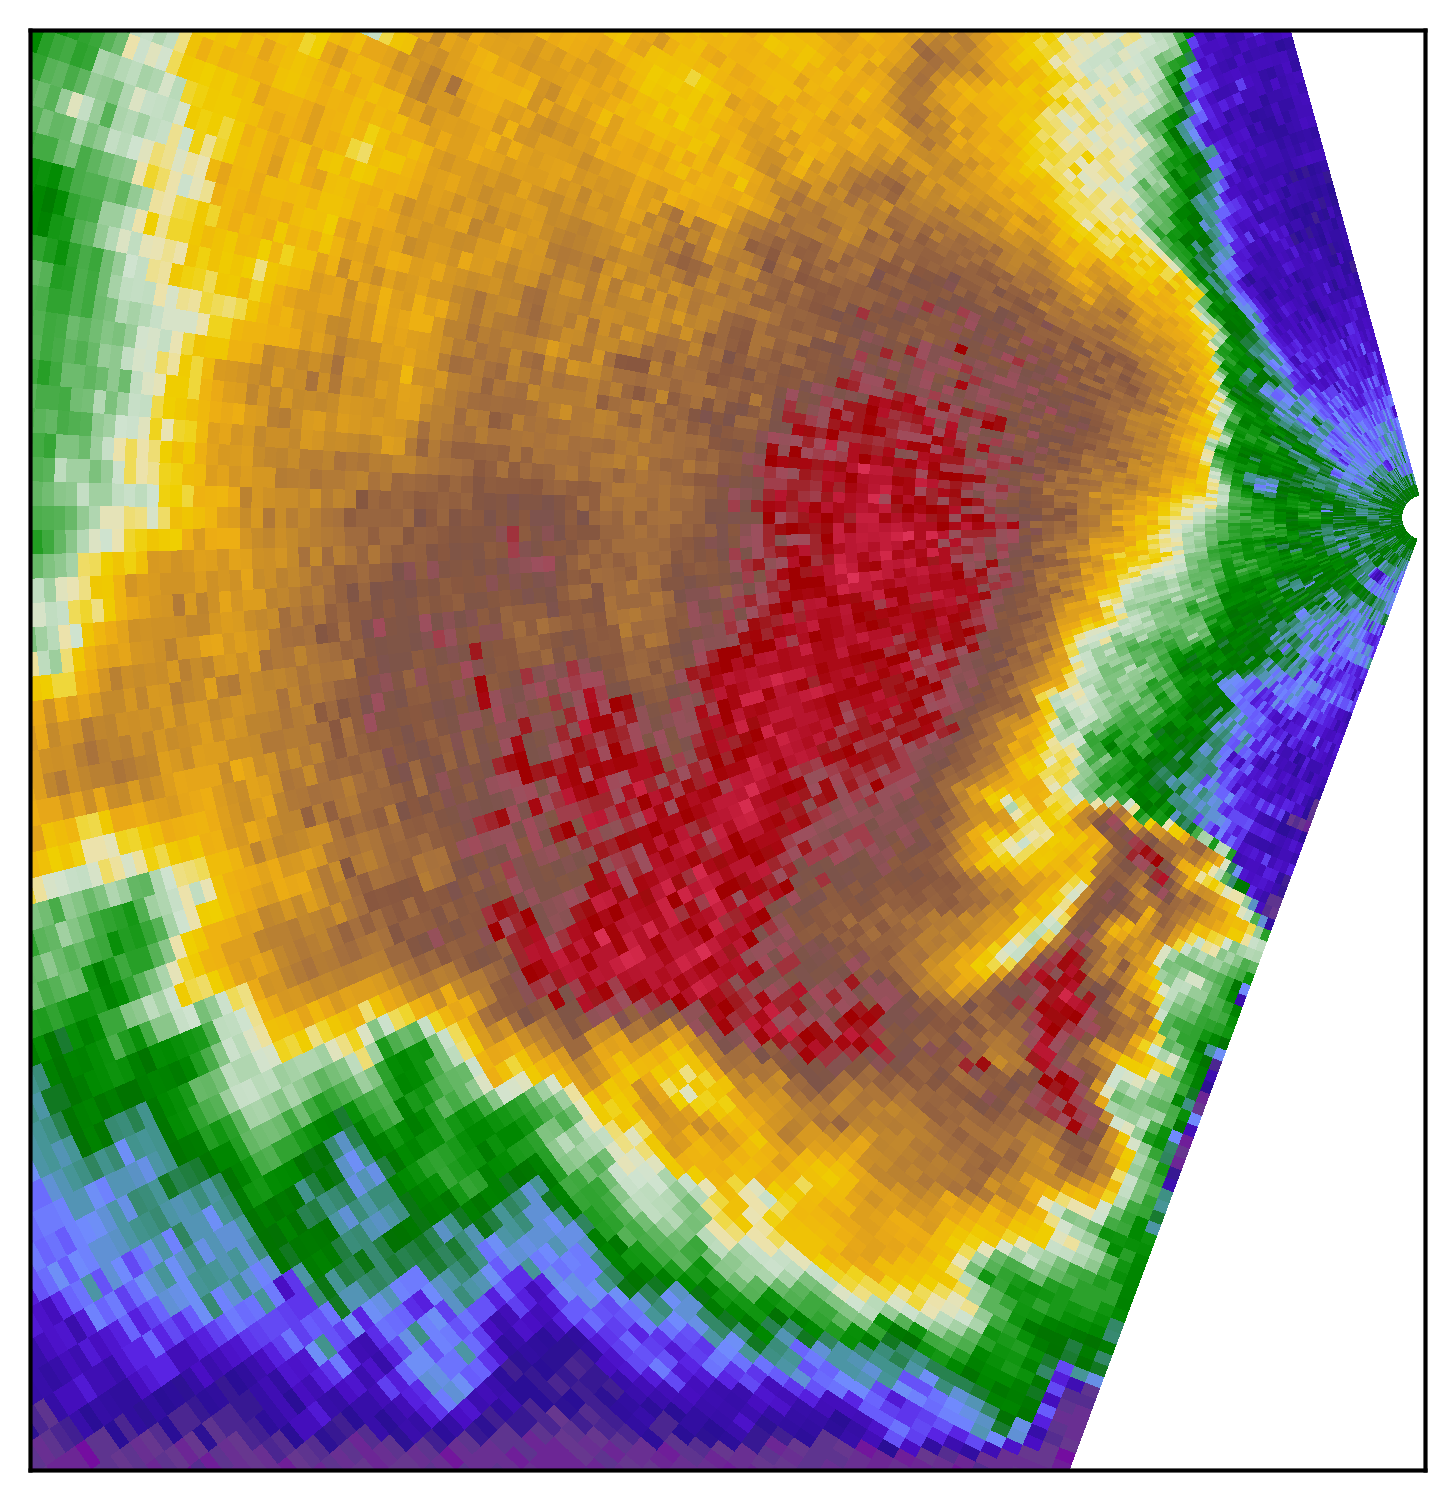
\includegraphics[scale=0.17]{figures/title_ppi.png}}

\begin{document}
\section{Backup}
\begin{frame}
	\begin{center}
		Backup Slides
	\end{center}
\end{frame}

\subsection{Model Errors}
\subsubsection{Control}
\begin{frame}
    \begin{center}
        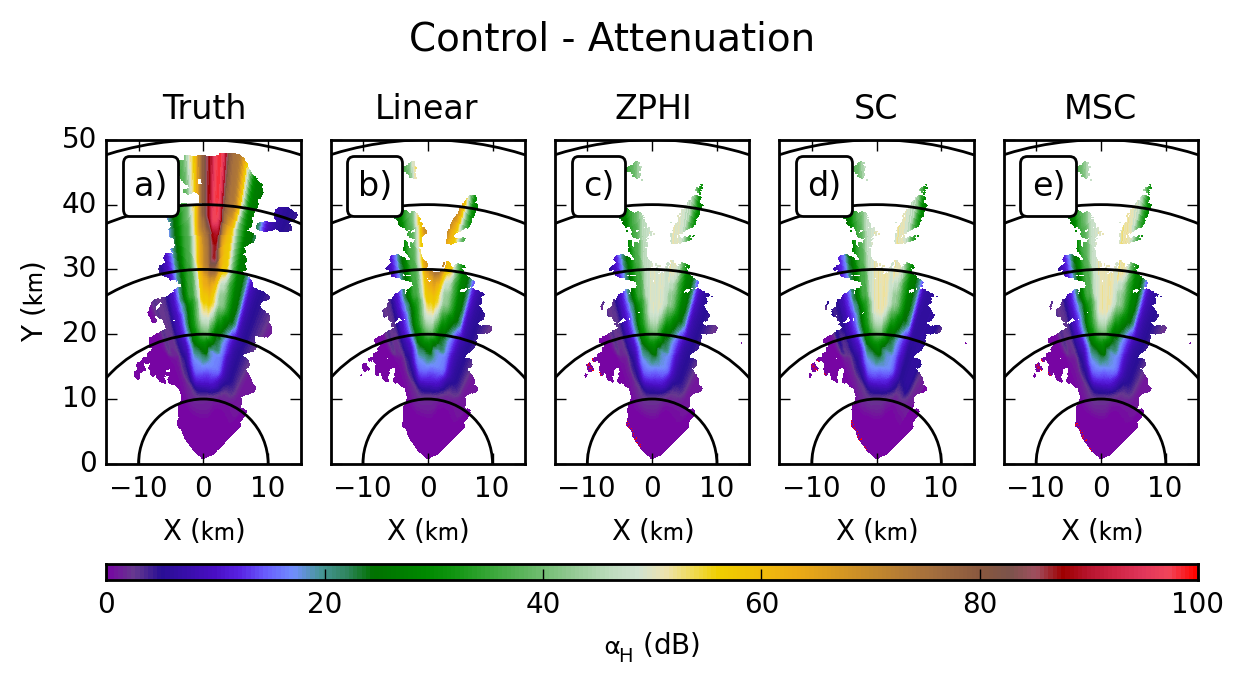
\includegraphics[scale=0.7]{figures/X_Control_Attenuation_H}
    \end{center}
\end{frame}

\begin{frame}
    \begin{center}
        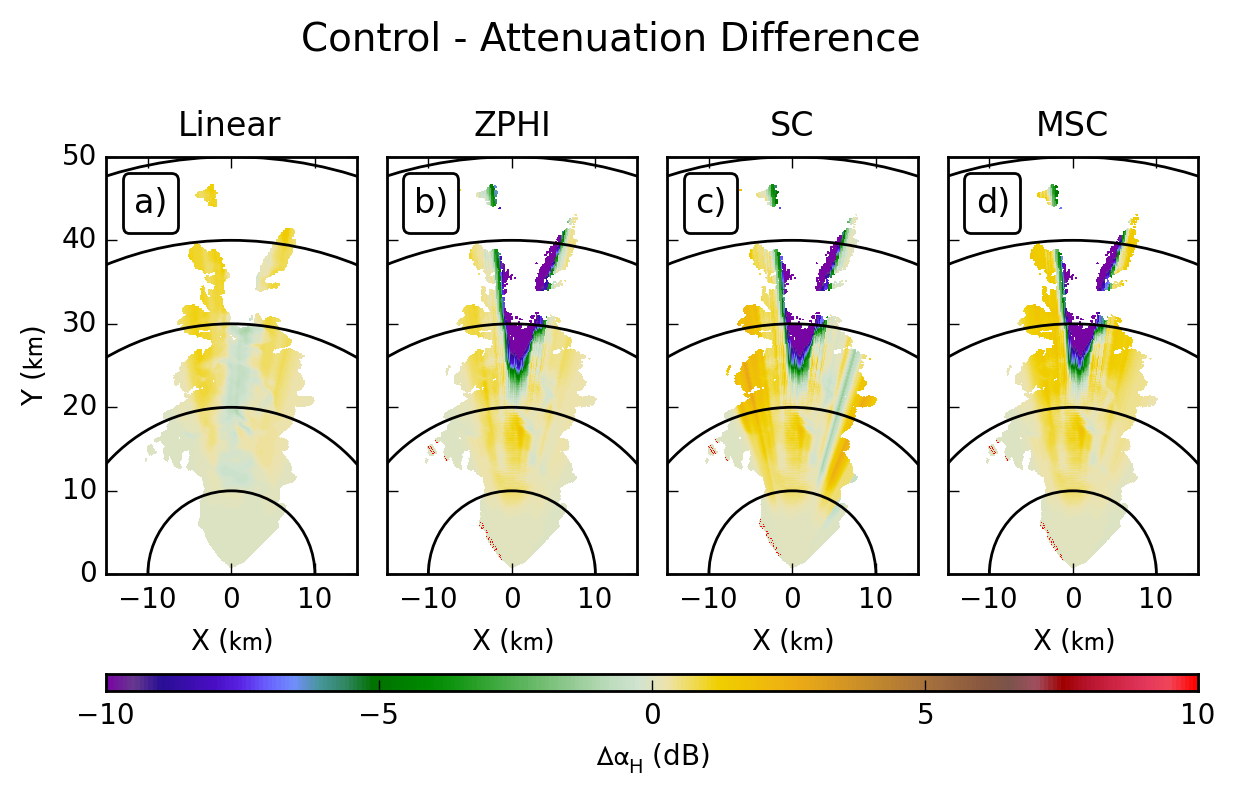
\includegraphics[scale=0.7]{figures/X_Control_Attenuation_Difference_H}
    \end{center}
\end{frame}

\begin{frame}
    \begin{center}
        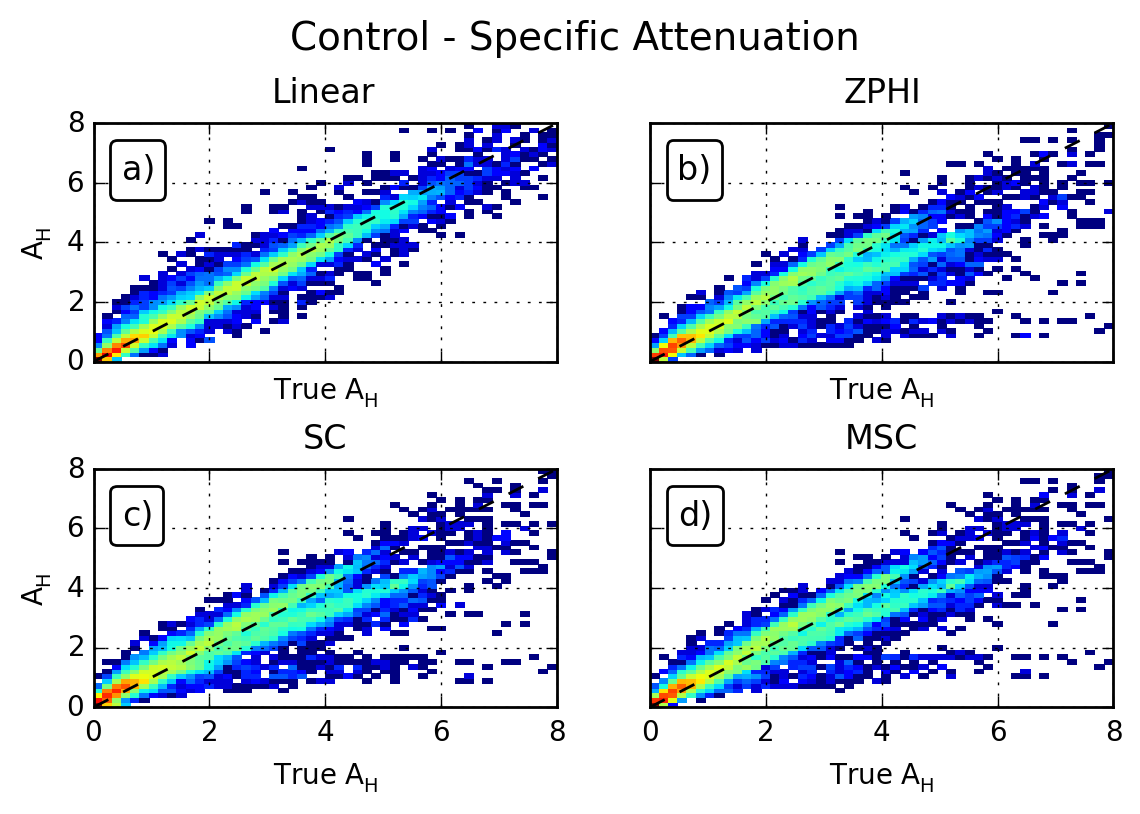
\includegraphics[scale=0.7]{figures/X_Control_Specific_Attenuation_H_scatter}
    \end{center}
\end{frame}

\begin{frame}
    \begin{center}
        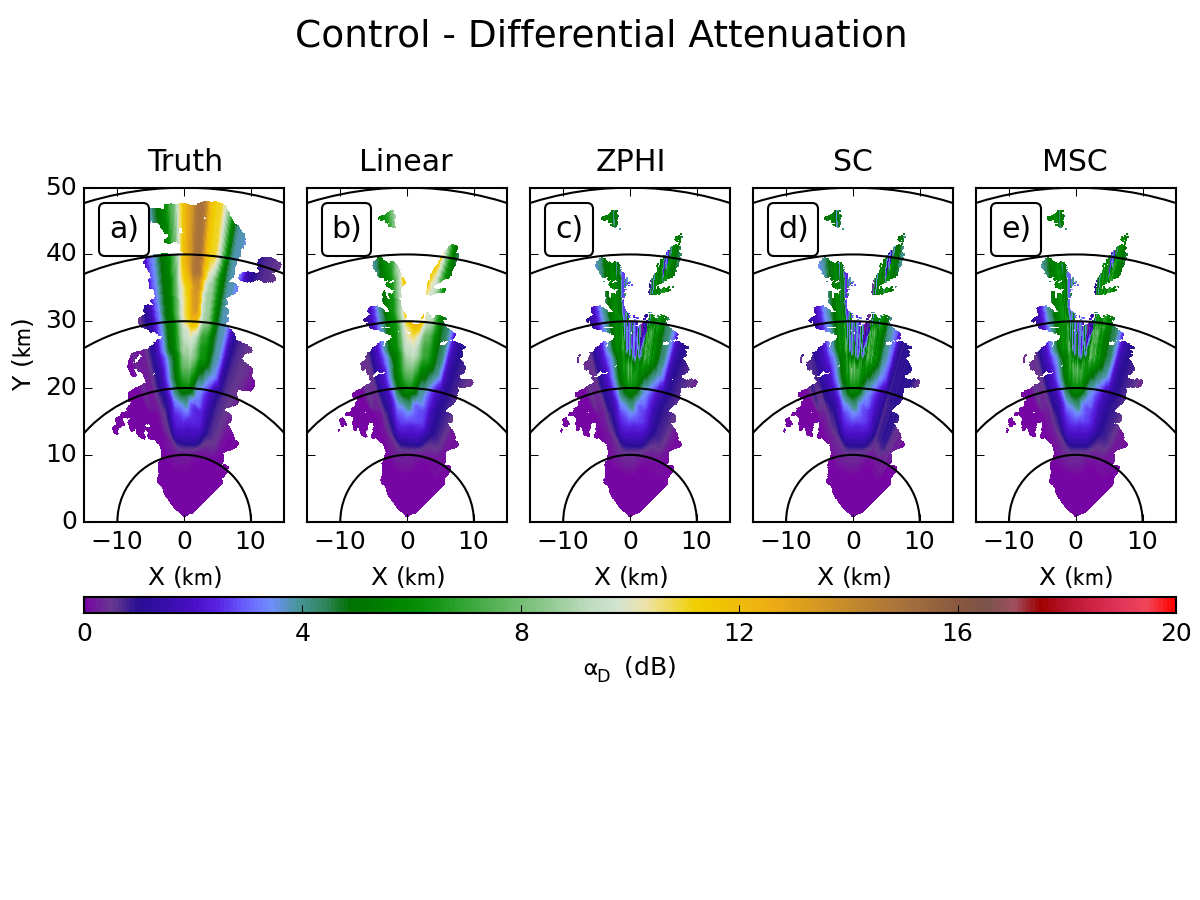
\includegraphics[scale=0.7]{figures/X_Control_Differential_Attenuation}
    \end{center}
\end{frame}

\begin{frame}
    \begin{center}
        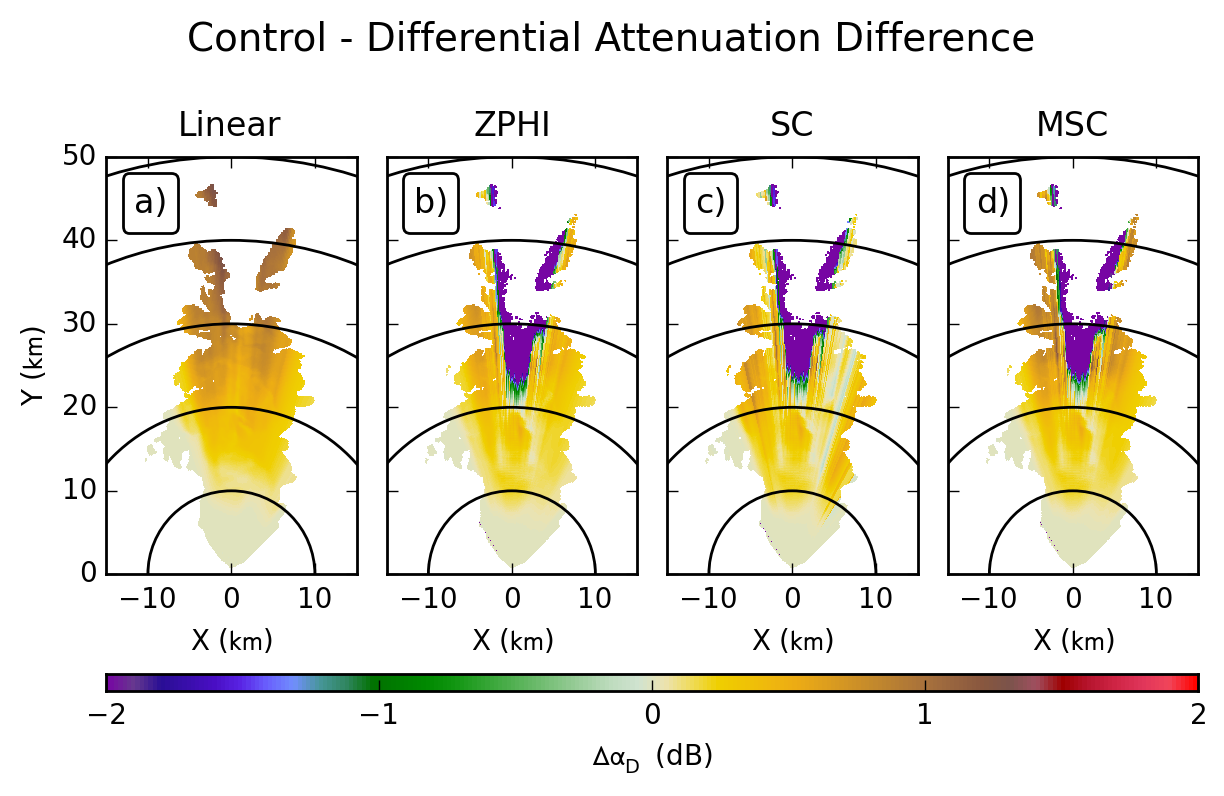
\includegraphics[scale=0.7]{figures/X_Control_Differential_Attenuation_Difference}
    \end{center}
\end{frame}

\begin{frame}
    \begin{center}
        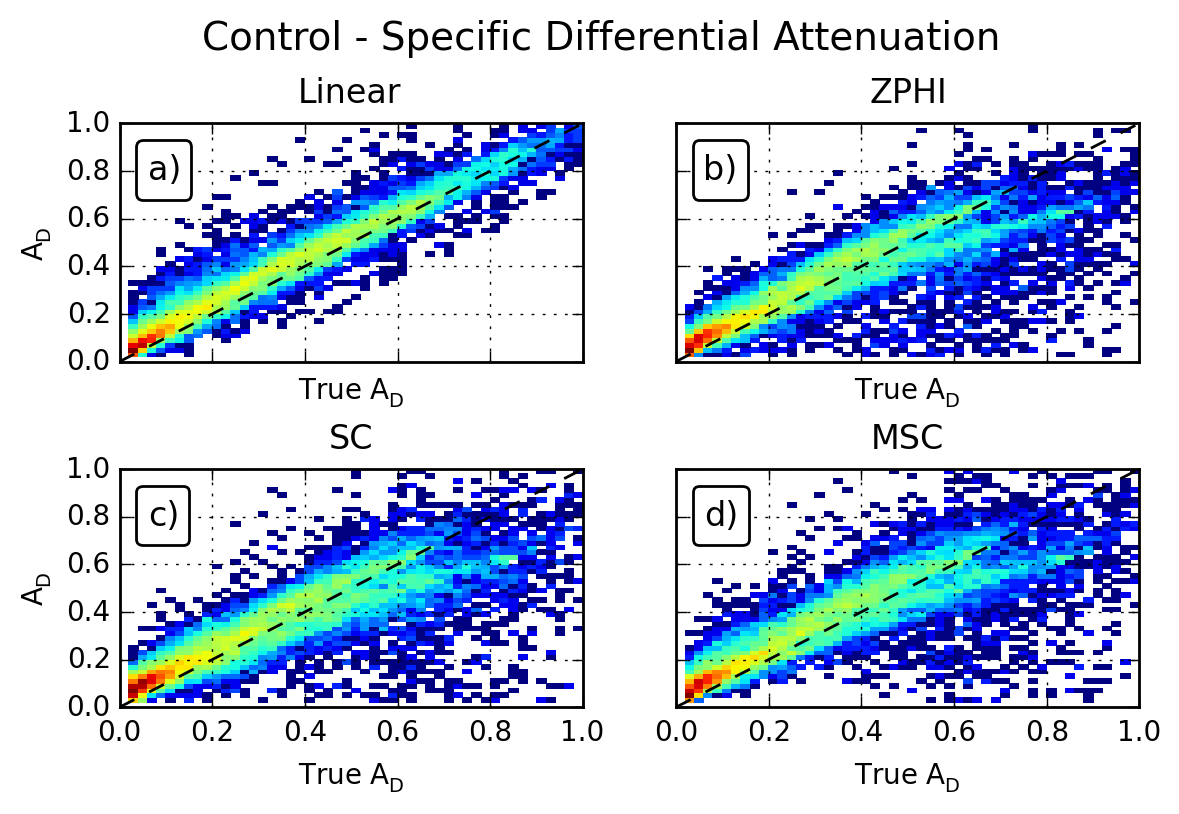
\includegraphics[scale=0.7]{figures/X_Control_Specific_Differential_Attenuation_scatter}
    \end{center}
\end{frame}

\subsubsection{Canting}
\begin{frame}
    \begin{center}
        \includegraphics<1>[scale=0.7]{figures/C_Canting_Attenuation_H}
        \includegraphics<2>[scale=0.7]{figures/C_Control_Attenuation_H}
    \end{center}
\end{frame}

\begin{frame}
    \begin{center}
        \includegraphics<1>[scale=0.7]{figures/C_Canting_Attenuation_Difference_H}
        \includegraphics<2>[scale=0.7]{figures/C_Control_Attenuation_Difference_H}
    \end{center}
\end{frame}

\begin{frame}
    \begin{center}
        \includegraphics<1>[scale=0.7]{figures/C_Canting_Specific_Attenuation_H_scatter}
        \includegraphics<2>[scale=0.7]{figures/C_Control_Specific_Attenuation_H_scatter}
    \end{center}
\end{frame}

\begin{frame}
    \begin{center}
        \includegraphics<1>[scale=0.7]{figures/C_Canting_Differential_Attenuation}
        \includegraphics<2>[scale=0.7]{figures/C_Control_Differential_Attenuation}
    \end{center}
\end{frame}

\begin{frame}
    \begin{center}
        \includegraphics<1>[scale=0.7]{figures/C_Canting_Differential_Attenuation_Difference}
        \includegraphics<2>[scale=0.7]{figures/C_Control_Differential_Attenuation_Difference}
    \end{center}
\end{frame}

\begin{frame}
    \begin{center}
        \includegraphics<1>[scale=0.7]{figures/C_Canting_Specific_Differential_Attenuation_scatter}
        \includegraphics<2>[scale=0.7]{figures/C_Control_Specific_Differential_Attenuation_scatter}
    \end{center}
\end{frame}

\begin{frame}
    \begin{center}
        \includegraphics<1>[scale=0.7]{figures/X_Canting_Attenuation_H}
        \includegraphics<2>[scale=0.7]{figures/X_Control_Attenuation_H}
    \end{center}
\end{frame}

\begin{frame}
    \begin{center}
        \includegraphics<1>[scale=0.7]{figures/X_Canting_Attenuation_Difference_H}
        \includegraphics<2>[scale=0.7]{figures/X_Control_Attenuation_Difference_H}
    \end{center}
\end{frame}

\begin{frame}
    \begin{center}
        \includegraphics<1>[scale=0.7]{figures/X_Canting_Specific_Attenuation_H_scatter}
        \includegraphics<2>[scale=0.7]{figures/X_Control_Specific_Attenuation_H_scatter}
    \end{center}
\end{frame}

\begin{frame}
    \begin{center}
        \includegraphics<1>[scale=0.7]{figures/X_Canting_Differential_Attenuation}
        \includegraphics<2>[scale=0.7]{figures/X_Control_Differential_Attenuation}
    \end{center}
\end{frame}

\begin{frame}
    \begin{center}
        \includegraphics<1>[scale=0.7]{figures/X_Canting_Differential_Attenuation_Difference}
        \includegraphics<2>[scale=0.7]{figures/X_Control_Differential_Attenuation_Difference}
    \end{center}
\end{frame}

\begin{frame}
    \begin{center}
        \includegraphics<1>[scale=0.7]{figures/X_Canting_Specific_Differential_Attenuation_scatter}
        \includegraphics<2>[scale=0.7]{figures/X_Control_Specific_Differential_Attenuation_scatter}
    \end{center}
\end{frame}

\subsubsection{Shape}
\begin{frame}
	\frametitle{Shape}
	\begin{center}
	    \begin{tabular}{ | l | l | }
	        \hline
	        Temperature & \SI{283}{\kelvin} \\
	        Drop Shape Model & Pruppacher \\
	        Wavelength & \SI{5.5}{\centi\meter}, \SI{3.21}{\centi\meter} \\
			\hline
	    \end{tabular}
	\end{center}	
\end{frame}

\begin{frame}
    \begin{center}
        \includegraphics<1>[scale=0.7]{figures/C_Shape_Attenuation_H}
        \includegraphics<2>[scale=0.7]{figures/C_Control_Attenuation_H}
    \end{center}
\end{frame}

\begin{frame}
    \begin{center}
        \includegraphics<1>[scale=0.7]{figures/C_Shape_Attenuation_Difference_H}
        \includegraphics<2>[scale=0.7]{figures/C_Control_Attenuation_Difference_H}
    \end{center}
\end{frame}

\begin{frame}
    \begin{center}
        \includegraphics<1>[scale=0.7]{figures/C_Shape_Specific_Attenuation_H_scatter}
        \includegraphics<2>[scale=0.7]{figures/C_Control_Specific_Attenuation_H_scatter}
    \end{center}
\end{frame}

\begin{frame}
    \begin{center}
        \includegraphics<1>[scale=0.7]{figures/C_Shape_Differential_Attenuation}
        \includegraphics<2>[scale=0.7]{figures/C_Control_Differential_Attenuation}
    \end{center}
\end{frame}

\begin{frame}
    \begin{center}
        \includegraphics<1>[scale=0.7]{figures/C_Shape_Differential_Attenuation_Difference}
        \includegraphics<2>[scale=0.7]{figures/C_Control_Differential_Attenuation_Difference}
    \end{center}
\end{frame}

\begin{frame}
    \begin{center}
        \includegraphics<1>[scale=0.7]{figures/C_Shape_Specific_Differential_Attenuation_scatter}
        \includegraphics<2>[scale=0.7]{figures/C_Control_Specific_Differential_Attenuation_scatter}
    \end{center}
\end{frame}

\begin{frame}
    \begin{center}
        \includegraphics<1>[scale=0.7]{figures/X_Shape_Attenuation_H}
        \includegraphics<2>[scale=0.7]{figures/X_Control_Attenuation_H}
    \end{center}
\end{frame}

\begin{frame}
    \begin{center}
        \includegraphics<1>[scale=0.7]{figures/X_Shape_Attenuation_Difference_H}
        \includegraphics<2>[scale=0.7]{figures/X_Control_Attenuation_Difference_H}
    \end{center}
\end{frame}

\begin{frame}
    \begin{center}
        \includegraphics<1>[scale=0.7]{figures/X_Shape_Specific_Attenuation_H_scatter}
        \includegraphics<2>[scale=0.7]{figures/X_Control_Specific_Attenuation_H_scatter}
    \end{center}
\end{frame}

\begin{frame}
    \begin{center}
        \includegraphics<1>[scale=0.7]{figures/X_Shape_Differential_Attenuation}
        \includegraphics<2>[scale=0.7]{figures/X_Control_Differential_Attenuation}
    \end{center}
\end{frame}

\begin{frame}
    \begin{center}
        \includegraphics<1>[scale=0.7]{figures/X_Shape_Differential_Attenuation_Difference}
        \includegraphics<2>[scale=0.7]{figures/X_Control_Differential_Attenuation_Difference}
    \end{center}
\end{frame}

\begin{frame}
    \begin{center}
        \includegraphics<1>[scale=0.7]{figures/X_Shape_Specific_Differential_Attenuation_scatter}
        \includegraphics<2>[scale=0.7]{figures/X_Control_Specific_Differential_Attenuation_scatter}
    \end{center}
\end{frame}

\subsubsection{Temperature}
\begin{frame}
    \begin{center}
        \includegraphics<1>[scale=0.7]{figures/C_Temperature_Attenuation_H}
        \includegraphics<2>[scale=0.7]{figures/C_Control_Attenuation_H}
    \end{center}
\end{frame}

\begin{frame}
    \begin{center}
        \includegraphics<1>[scale=0.7]{figures/C_Temperature_Differential_Attenuation}
        \includegraphics<2>[scale=0.7]{figures/C_Control_Differential_Attenuation}
    \end{center}
\end{frame}

\begin{frame}
    \begin{center}
        \includegraphics<1>[scale=0.7]{figures/X_Temperature_Attenuation_H}
        \includegraphics<2>[scale=0.7]{figures/X_Control_Attenuation_H}
    \end{center}
\end{frame}

\begin{frame}
    \begin{center}
        \includegraphics<1>[scale=0.7]{figures/X_Temperature_Attenuation_Difference_H}
        \includegraphics<2>[scale=0.7]{figures/X_Control_Attenuation_Difference_H}
    \end{center}
\end{frame}

\begin{frame}
    \begin{center}
        \includegraphics<1>[scale=0.7]{figures/X_Temperature_Specific_Attenuation_H_scatter}
        \includegraphics<2>[scale=0.7]{figures/X_Control_Specific_Attenuation_H_scatter}
    \end{center}
\end{frame}

\begin{frame}
    \begin{center}
        \includegraphics<1>[scale=0.7]{figures/X_Temperature_Differential_Attenuation}
        \includegraphics<2>[scale=0.7]{figures/X_Control_Differential_Attenuation}
    \end{center}
\end{frame}

\begin{frame}
    \begin{center}
        \includegraphics<1>[scale=0.7]{figures/X_Temperature_Differential_Attenuation_Difference}
        \includegraphics<2>[scale=0.7]{figures/X_Control_Differential_Attenuation_Difference}
    \end{center}
\end{frame}

\begin{frame}
    \begin{center}
        \includegraphics<1>[scale=0.7]{figures/X_Temperature_Specific_Differential_Attenuation_scatter}
        \includegraphics<2>[scale=0.7]{figures/X_Control_Specific_Differential_Attenuation_scatter}
    \end{center}
\end{frame}

\subsubsection{Wavelength}
\begin{frame}
    \begin{center}
        \includegraphics<1>[scale=0.7]{figures/C_Wavelength_Attenuation_H}
        \includegraphics<2>[scale=0.7]{figures/C_Control_Attenuation_H}
    \end{center}
\end{frame}

\begin{frame}
    \begin{center}
        \includegraphics<1>[scale=0.7]{figures/C_Wavelength_Differential_Attenuation}
        \includegraphics<2>[scale=0.7]{figures/C_Control_Differential_Attenuation}
    \end{center}
\end{frame}

\begin{frame}
    \begin{center}
        \includegraphics<1>[scale=0.7]{figures/X_Wavelength_Attenuation_H}
        \includegraphics<2>[scale=0.7]{figures/X_Control_Attenuation_H}
    \end{center}
\end{frame}

\begin{frame}
    \begin{center}
        \includegraphics<1>[scale=0.7]{figures/X_Wavelength_Attenuation_Difference_H}
        \includegraphics<2>[scale=0.7]{figures/X_Control_Attenuation_Difference_H}
    \end{center}
\end{frame}

\begin{frame}
    \begin{center}
        \includegraphics<1>[scale=0.7]{figures/X_Wavelength_Specific_Attenuation_H_scatter}
        \includegraphics<2>[scale=0.7]{figures/X_Control_Specific_Attenuation_H_scatter}
    \end{center}
\end{frame}

\begin{frame}
    \begin{center}
        \includegraphics<1>[scale=0.7]{figures/X_Wavelength_Differential_Attenuation}
        \includegraphics<2>[scale=0.7]{figures/X_Control_Differential_Attenuation}
    \end{center}
\end{frame}

\begin{frame}
    \begin{center}
        \includegraphics<1>[scale=0.7]{figures/X_Wavelength_Differential_Attenuation_Difference}
        \includegraphics<2>[scale=0.7]{figures/X_Control_Differential_Attenuation_Difference}
    \end{center}
\end{frame}

\begin{frame}
    \begin{center}
        \includegraphics<1>[scale=0.7]{figures/X_Wavelength_Specific_Differential_Attenuation_scatter}
        \includegraphics<2>[scale=0.7]{figures/X_Control_Specific_Differential_Attenuation_scatter}
    \end{center}
\end{frame}

\subsubsection{Combined}
\begin{frame}
	\frametitle{Worst Case}
	\begin{center}
	    \begin{tabular}{ | l | l | }
	        \hline
	        Temperature & Model Field (\textasciitilde\SI{293}{\kelvin}) \\
	        Drop Shape Model & Pruppacher \\
	        Wavelength & \SI{5.0}{\centi\meter} \\
			\hline
	    \end{tabular}
	\end{center}	
\end{frame}

\begin{frame}
    \begin{center}
        \includegraphics<1>[scale=0.7]{figures/C_Combined_Attenuation_H}
        \includegraphics<2>[scale=0.7]{figures/C_Control_Attenuation_H}
    \end{center}
\end{frame}

\begin{frame}
    \begin{center}
        \includegraphics<1>[scale=0.7]{figures/C_Combined_Attenuation_Difference_H}
        \includegraphics<2>[scale=0.7]{figures/C_Control_Attenuation_Difference_H}
    \end{center}
\end{frame}

\begin{frame}
    \begin{center}
        \includegraphics<1>[scale=0.7]{figures/C_Combined_Specific_Attenuation_H_scatter}
        \includegraphics<2>[scale=0.7]{figures/C_Control_Specific_Attenuation_H_scatter}
    \end{center}
\end{frame}

\begin{frame}
    \begin{center}
        \includegraphics<1>[scale=0.7]{figures/C_Combined_Differential_Attenuation}
        \includegraphics<2>[scale=0.7]{figures/C_Control_Differential_Attenuation}
    \end{center}
\end{frame}

\begin{frame}
    \begin{center}
        \includegraphics<1>[scale=0.7]{figures/C_Combined_Differential_Attenuation_Difference}
        \includegraphics<2>[scale=0.7]{figures/C_Control_Differential_Attenuation_Difference}
    \end{center}
\end{frame}

\begin{frame}
    \begin{center}
        \includegraphics<1>[scale=0.7]{figures/C_Combined_Specific_Differential_Attenuation_scatter}
        \includegraphics<2>[scale=0.7]{figures/C_Control_Specific_Differential_Attenuation_scatter}
    \end{center}
\end{frame}

\begin{frame}
    \begin{center}
        \includegraphics<1>[scale=0.7]{figures/X_Combined_Attenuation_H}
        \includegraphics<2>[scale=0.7]{figures/X_Control_Attenuation_H}
    \end{center}
\end{frame}

\begin{frame}
    \begin{center}
        \includegraphics<1>[scale=0.7]{figures/X_Combined_Attenuation_Difference_H}
        \includegraphics<2>[scale=0.7]{figures/X_Control_Attenuation_Difference_H}
    \end{center}
\end{frame}

\begin{frame}
    \begin{center}
        \includegraphics<1>[scale=0.7]{figures/X_Combined_Specific_Attenuation_H_scatter}
        \includegraphics<2>[scale=0.7]{figures/X_Control_Specific_Attenuation_H_scatter}
    \end{center}
\end{frame}

\begin{frame}
    \begin{center}
        \includegraphics<1>[scale=0.7]{figures/X_Combined_Differential_Attenuation}
        \includegraphics<2>[scale=0.7]{figures/X_Control_Differential_Attenuation}
    \end{center}
\end{frame}

\begin{frame}
    \begin{center}
        \includegraphics<1>[scale=0.7]{figures/X_Combined_Differential_Attenuation_Difference}
        \includegraphics<2>[scale=0.7]{figures/X_Control_Differential_Attenuation_Difference}
    \end{center}
\end{frame}

\begin{frame}
    \begin{center}
        \includegraphics<1>[scale=0.7]{figures/X_Combined_Specific_Differential_Attenuation_scatter}
        \includegraphics<2>[scale=0.7]{figures/X_Control_Specific_Differential_Attenuation_scatter}
    \end{center}
\end{frame}

\subsubsection{Vertical Channel}
\begin{frame}
    \begin{center}
        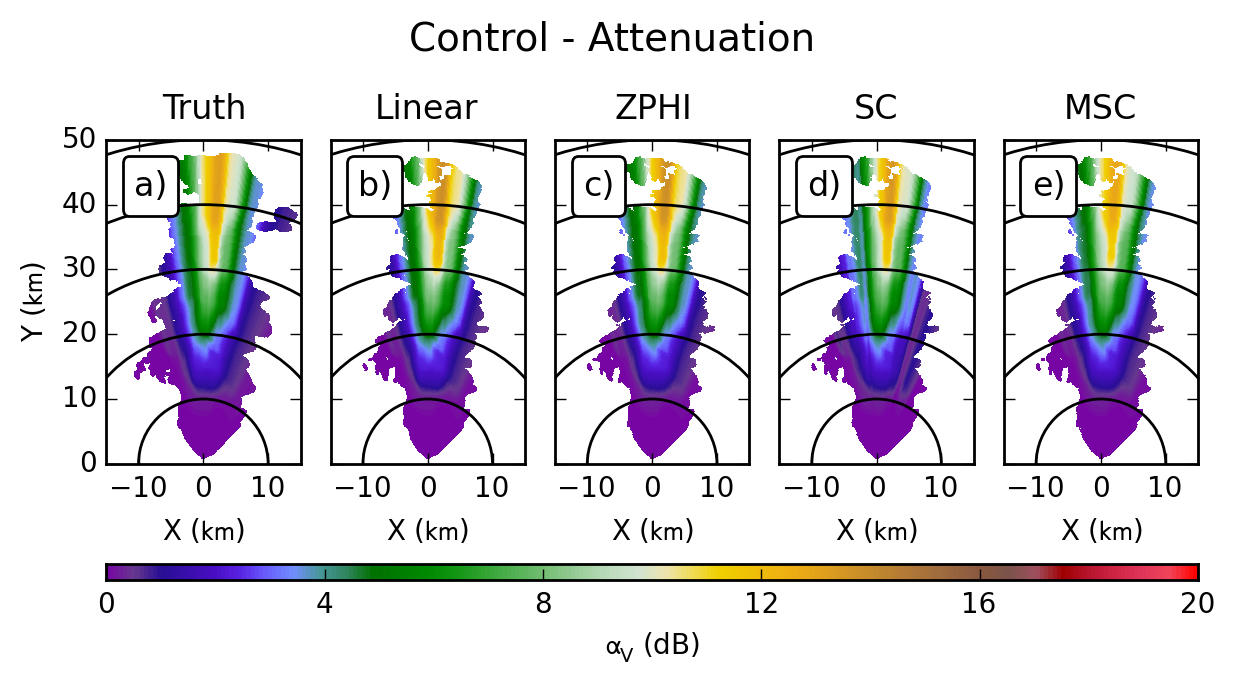
\includegraphics[scale=0.7]{figures/C_Control_Attenuation_V}
    \end{center}
\end{frame}

\begin{frame}
    \begin{center}
        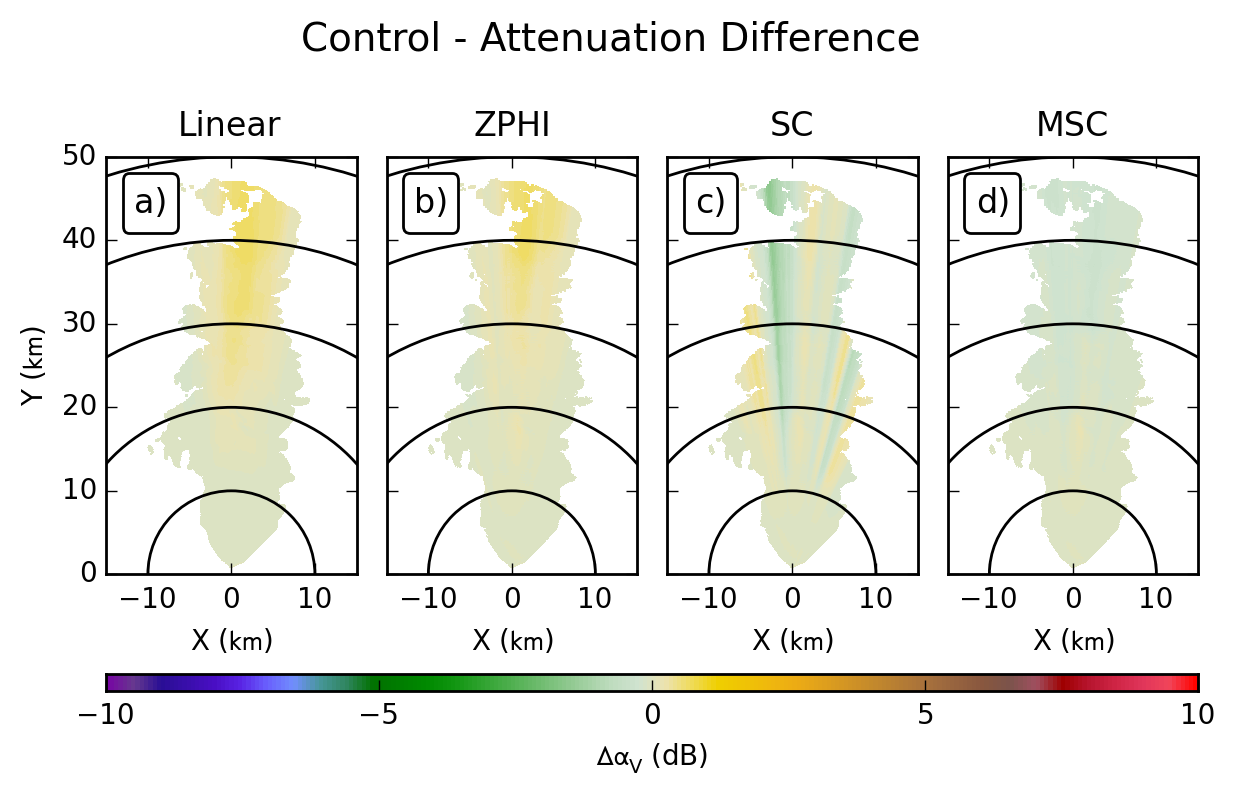
\includegraphics[scale=0.7]{figures/C_Control_Attenuation_Difference_V}
    \end{center}
\end{frame}

\begin{frame}
    \begin{center}
        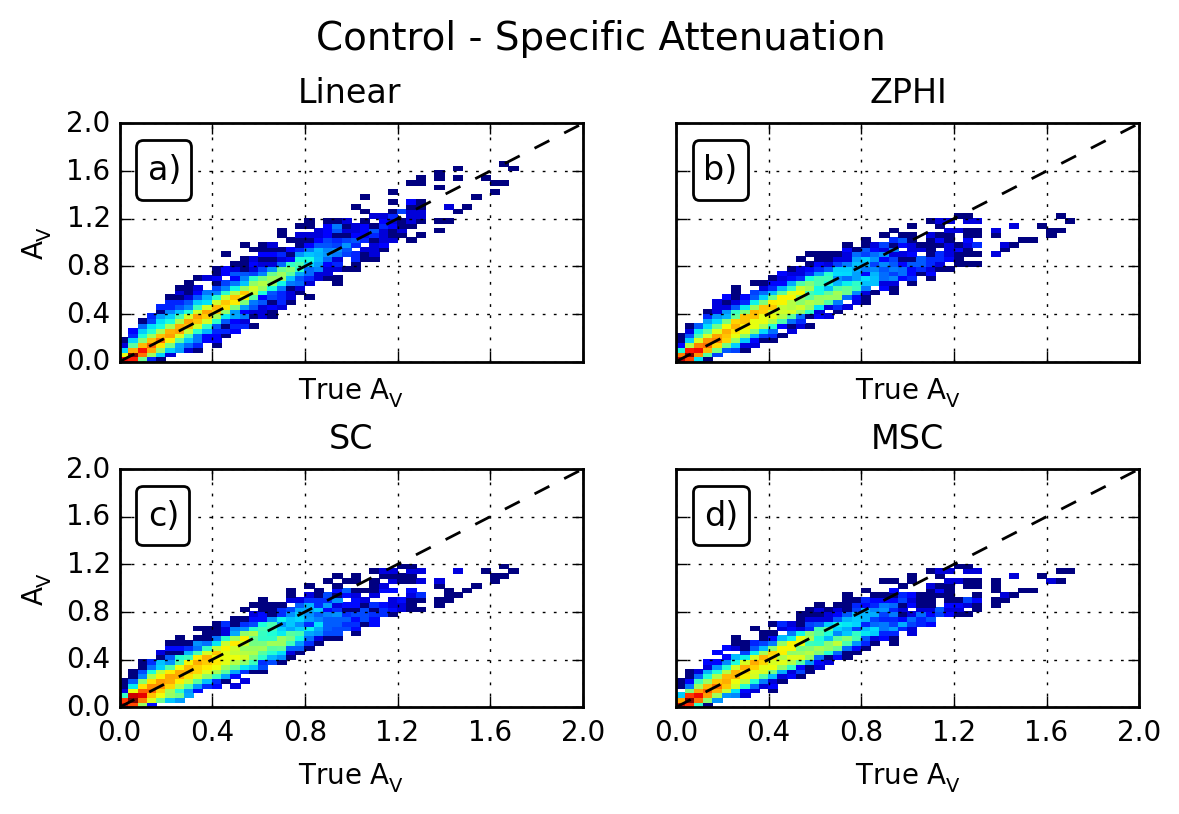
\includegraphics[scale=0.7]{figures/C_Control_Specific_Attenuation_V_scatter}
    \end{center}
\end{frame}

\begin{frame}
    \begin{center}
        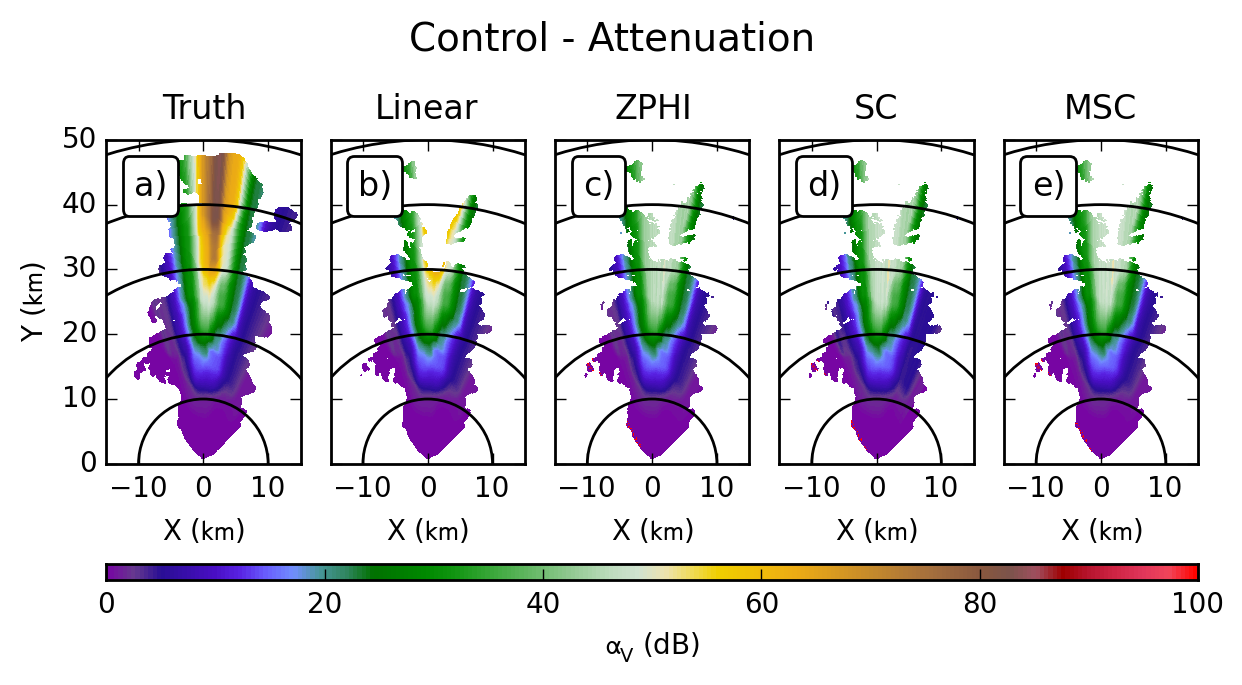
\includegraphics[scale=0.7]{figures/X_Control_Attenuation_V}
    \end{center}
\end{frame}

\begin{frame}
    \begin{center}
        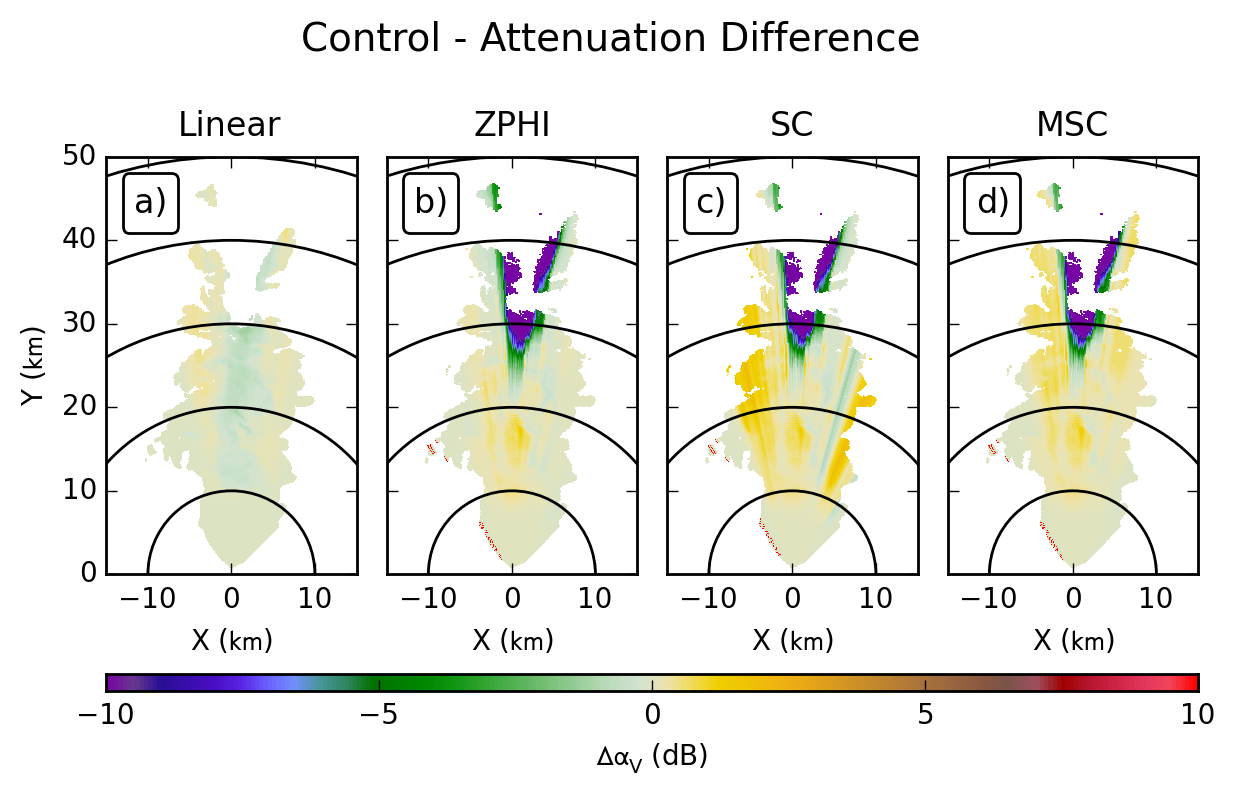
\includegraphics[scale=0.7]{figures/X_Control_Attenuation_Difference_V}
    \end{center}
\end{frame}

\begin{frame}
    \begin{center}
        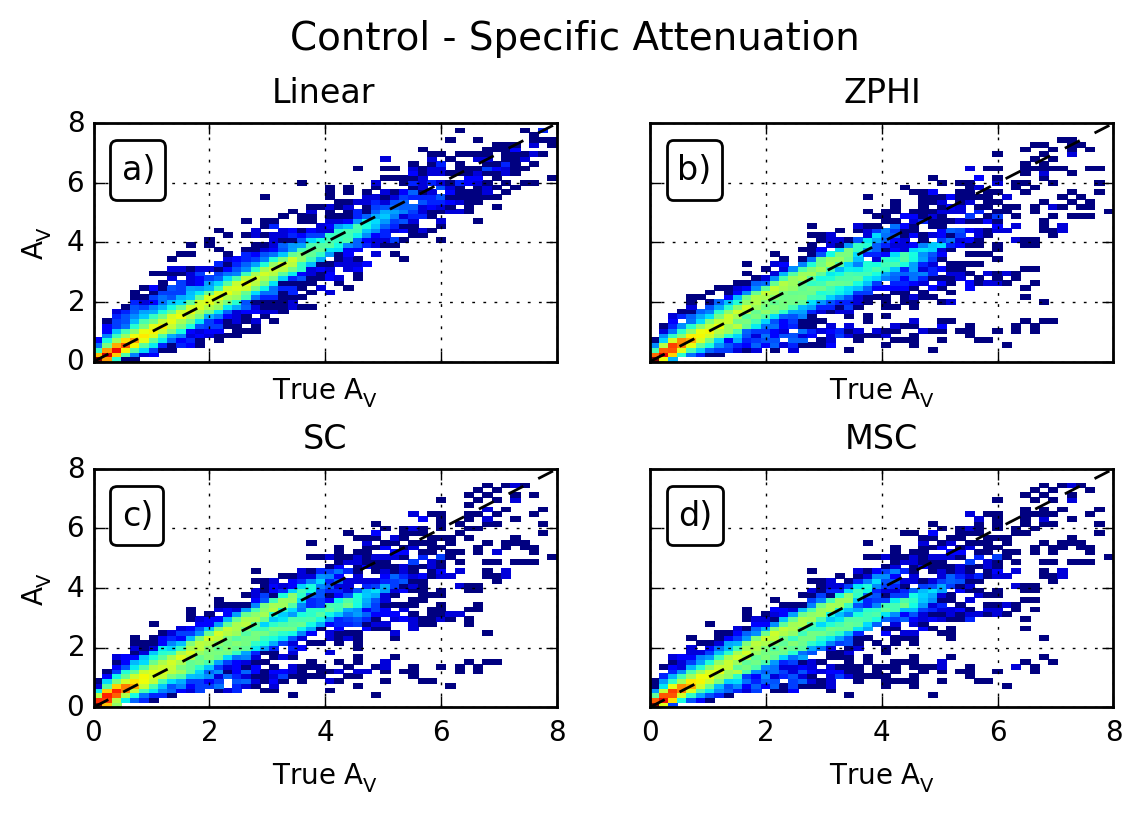
\includegraphics[scale=0.7]{figures/X_Control_Specific_Attenuation_V_scatter}
    \end{center}
\end{frame}

\begin{frame}
    \begin{center}
        \includegraphics<1>[scale=0.7]{figures/C_Canting_Attenuation_V}
        \includegraphics<2>[scale=0.7]{figures/C_Control_Attenuation_V}
    \end{center}
\end{frame}

\begin{frame}
    \begin{center}
        \includegraphics<1>[scale=0.7]{figures/C_Canting_Attenuation_Difference_V}
        \includegraphics<2>[scale=0.7]{figures/C_Control_Attenuation_Difference_V}
    \end{center}
\end{frame}

\begin{frame}
    \begin{center}
        \includegraphics<1>[scale=0.7]{figures/C_Canting_Specific_Attenuation_V_scatter}
        \includegraphics<2>[scale=0.7]{figures/C_Control_Specific_Attenuation_V_scatter}
    \end{center}
\end{frame}

\begin{frame}
    \begin{center}
        \includegraphics<1>[scale=0.7]{figures/X_Canting_Attenuation_V}
        \includegraphics<2>[scale=0.7]{figures/X_Control_Attenuation_V}
    \end{center}
\end{frame}

\begin{frame}
    \begin{center}
        \includegraphics<1>[scale=0.7]{figures/X_Canting_Attenuation_Difference_V}
        \includegraphics<2>[scale=0.7]{figures/X_Control_Attenuation_Difference_V}
    \end{center}
\end{frame}

\begin{frame}
    \begin{center}
        \includegraphics<1>[scale=0.7]{figures/X_Canting_Specific_Attenuation_V_scatter}
        \includegraphics<2>[scale=0.7]{figures/X_Control_Specific_Attenuation_V_scatter}
    \end{center}
\end{frame}

\begin{frame}
    \begin{center}
        \includegraphics<1>[scale=0.7]{figures/C_Shape_Attenuation_V}
        \includegraphics<2>[scale=0.7]{figures/C_Control_Attenuation_V}
    \end{center}
\end{frame}

\begin{frame}
    \begin{center}
        \includegraphics<1>[scale=0.7]{figures/C_Shape_Attenuation_Difference_V}
        \includegraphics<2>[scale=0.7]{figures/C_Control_Attenuation_Difference_V}
    \end{center}
\end{frame}

\begin{frame}
    \begin{center}
        \includegraphics<1>[scale=0.7]{figures/C_Shape_Specific_Attenuation_V_scatter}
        \includegraphics<2>[scale=0.7]{figures/C_Control_Specific_Attenuation_V_scatter}
    \end{center}
\end{frame}

\begin{frame}
    \begin{center}
        \includegraphics<1>[scale=0.7]{figures/X_Shape_Attenuation_V}
        \includegraphics<2>[scale=0.7]{figures/X_Control_Attenuation_V}
    \end{center}
\end{frame}

\begin{frame}
    \begin{center}
        \includegraphics<1>[scale=0.7]{figures/X_Shape_Attenuation_Difference_V}
        \includegraphics<2>[scale=0.7]{figures/X_Control_Attenuation_Difference_V}
    \end{center}
\end{frame}

\begin{frame}
    \begin{center}
        \includegraphics<1>[scale=0.7]{figures/X_Shape_Specific_Attenuation_V_scatter}
        \includegraphics<2>[scale=0.7]{figures/X_Control_Specific_Attenuation_V_scatter}
    \end{center}
\end{frame}

\begin{frame}
    \begin{center}
        \includegraphics<1>[scale=0.7]{figures/C_Temperature_Attenuation_V}
        \includegraphics<2>[scale=0.7]{figures/C_Control_Attenuation_V}
    \end{center}
\end{frame}

\begin{frame}
    \begin{center}
        \includegraphics<1>[scale=0.7]{figures/C_Temperature_Attenuation_Difference_V}
        \includegraphics<2>[scale=0.7]{figures/C_Control_Attenuation_Difference_V}
    \end{center}
\end{frame}

\begin{frame}
    \begin{center}
        \includegraphics<1>[scale=0.7]{figures/C_Temperature_Specific_Attenuation_V_scatter}
        \includegraphics<2>[scale=0.7]{figures/C_Control_Specific_Attenuation_V_scatter}
    \end{center}
\end{frame}

\begin{frame}
    \begin{center}
        \includegraphics<1>[scale=0.7]{figures/X_Temperature_Attenuation_V}
        \includegraphics<2>[scale=0.7]{figures/X_Control_Attenuation_V}
    \end{center}
\end{frame}

\begin{frame}
    \begin{center}
        \includegraphics<1>[scale=0.7]{figures/X_Temperature_Attenuation_Difference_V}
        \includegraphics<2>[scale=0.7]{figures/X_Control_Attenuation_Difference_V}
    \end{center}
\end{frame}

\begin{frame}
    \begin{center}
        \includegraphics<1>[scale=0.7]{figures/X_Temperature_Specific_Attenuation_V_scatter}
        \includegraphics<2>[scale=0.7]{figures/X_Control_Specific_Attenuation_V_scatter}
    \end{center}
\end{frame}

\begin{frame}
    \begin{center}
        \includegraphics<1>[scale=0.7]{figures/C_Wavelength_Attenuation_V}
        \includegraphics<2>[scale=0.7]{figures/C_Control_Attenuation_V}
    \end{center}
\end{frame}

\begin{frame}
    \begin{center}
        \includegraphics<1>[scale=0.7]{figures/C_Wavelength_Attenuation_Difference_V}
        \includegraphics<2>[scale=0.7]{figures/C_Control_Attenuation_Difference_V}
    \end{center}
\end{frame}

\begin{frame}
    \begin{center}
        \includegraphics<1>[scale=0.7]{figures/C_Wavelength_Specific_Attenuation_V_scatter}
        \includegraphics<2>[scale=0.7]{figures/C_Control_Specific_Attenuation_V_scatter}
    \end{center}
\end{frame}

\begin{frame}
    \begin{center}
        \includegraphics<1>[scale=0.7]{figures/X_Wavelength_Attenuation_V}
        \includegraphics<2>[scale=0.7]{figures/X_Control_Attenuation_V}
    \end{center}
\end{frame}

\begin{frame}
    \begin{center}
        \includegraphics<1>[scale=0.7]{figures/X_Wavelength_Attenuation_Difference_V}
        \includegraphics<2>[scale=0.7]{figures/X_Control_Attenuation_Difference_V}
    \end{center}
\end{frame}

\begin{frame}
    \begin{center}
        \includegraphics<1>[scale=0.7]{figures/X_Wavelength_Specific_Attenuation_V_scatter}
        \includegraphics<2>[scale=0.7]{figures/X_Control_Specific_Attenuation_V_scatter}
    \end{center}
\end{frame}

\begin{frame}
    \begin{center}
        \includegraphics<1>[scale=0.7]{figures/C_Combined_Attenuation_V}
        \includegraphics<2>[scale=0.7]{figures/C_Control_Attenuation_V}
    \end{center}
\end{frame}

\begin{frame}
    \begin{center}
        \includegraphics<1>[scale=0.7]{figures/C_Combined_Attenuation_Difference_V}
        \includegraphics<2>[scale=0.7]{figures/C_Control_Attenuation_Difference_V}
    \end{center}
\end{frame}

\begin{frame}
    \begin{center}
        \includegraphics<1>[scale=0.7]{figures/C_Combined_Specific_Attenuation_V_scatter}
        \includegraphics<2>[scale=0.7]{figures/C_Control_Specific_Attenuation_V_scatter}
    \end{center}
\end{frame}

\begin{frame}
    \begin{center}
        \includegraphics<1>[scale=0.7]{figures/X_Combined_Attenuation_V}
        \includegraphics<2>[scale=0.7]{figures/X_Control_Attenuation_V}
    \end{center}
\end{frame}

\begin{frame}
    \begin{center}
        \includegraphics<1>[scale=0.7]{figures/X_Combined_Attenuation_Difference_V}
        \includegraphics<2>[scale=0.7]{figures/X_Control_Attenuation_Difference_V}
    \end{center}
\end{frame}

\begin{frame}
    \begin{center}
        \includegraphics<1>[scale=0.7]{figures/X_Combined_Specific_Attenuation_V_scatter}
        \includegraphics<2>[scale=0.7]{figures/X_Control_Specific_Attenuation_V_scatter}
    \end{center}
\end{frame}

\begin{frame}
    \frametitle{Summary: MSE at C-band for Horizontal Polarization (\si{dB\squared\per \kilo\meter\squared})}
    \begin{center}
        \begin{tabular}{| c | c | c | c | c |}
            \hline
            Experiment & Linear & ZPHI & SC & MSC \\
            \hline
            \hline
            Control & 0.0047 & 0.0070 & 0.0070 & 0.0059 \\
            Canting & 0.0068 & 0.0094 & 0.0071 & 0.0060 \\
            Shape & 0.0251 & 0.0379 & 0.0079 & 0.0070 \\
            Temperature & 0.0191 & 0.0230 & 0.0062 & 0.0050 \\
            Wavelength & 0.0171 & 0.0259 & 0.0123 & 0.0117 \\
            Combined & 0.0302 & 0.0478 & 0.0132 & 0.0143 \\
            \hline
        \end{tabular}
    \end{center}
\end{frame}

\begin{frame}
    \frametitle{Summary: $r^2$ at C-band for Horizontal Polarization}
    \begin{center}
        \begin{tabular}{| c | c | c | c | c |}
            \hline
            Experiment & Linear & ZPHI & SC & MSC \\
            \hline
            \hline
            Control & 0.9612 & 0.9233 & 0.9173 & 0.9305 \\
            Canting & 0.9612 & 0.9136 & 0.9165 & 0.9306 \\
            Shape & 0.9560 & 0.8265 & 0.9083 & 0.9279 \\
            Temperature & 0.9554 & 0.8453 & 0.8974 & 0.9235 \\
            Wavelength & 0.9596 & 0.9002 & 0.9304 & 0.9351 \\
            Combined & 0.9418 & 0.8375 & 0.9128 & 0.9202 \\
            \hline
        \end{tabular}
    \end{center}
\end{frame}

\begin{frame}
    \frametitle{Summary: Bias at C-band for Vertical Polarization (\si{dB\per \kilo\meter})}
    \begin{center}
        \begin{tabular}{| c | c | c | c | c |}
            \hline
            Experiment & Linear & ZPHI & SC & MSC \\
            \hline
            \hline
            Control & 0.0095 & 0.0071 & -0.0027 & -0.0087 \\
            Canting & 0.0243 & 0.0214 & -0.0024 & -0.0096 \\
            Shape & 0.0819 & 0.0803 & 0.0070 & -0.0074 \\
            Temperature & 0.0727 & 0.0689 & -0.0022 & -0.0135 \\
            Wavelength & -0.0704 & -0.0701 & -0.0020 & -0.0063 \\
            Combined & 0.1050 & 0.1027 & 0.0107 & -0.0093 \\
            \hline
        \end{tabular}
    \end{center}
\end{frame}

\begin{frame}
    \frametitle{Summary: MSE at C-band for Vertical Polarization (\si{dB\squared\per \kilo\meter\squared})}
    \begin{center}
        \begin{tabular}{| c | c | c | c | c |}
            \hline
            Experiment & Linear & ZPHI & SC & MSC \\
            \hline
            \hline
            Control & 0.0020 & 0.0033 & 0.0042 & 0.0034 \\
            Canting & 0.0032 & 0.0041 & 0.0042 & 0.0034 \\
            Shape & 0.0128 & 0.0167 & 0.0040 & 0.0034 \\
            Temperature & 0.0111 & 0.0112 & 0.0036 & 0.0028 \\
            Wavelength & 0.0125 & 0.0191 & 0.0074 & 0.0069 \\
            Combined & 0.0187 & 0.0259 & 0.0063 & 0.0065 \\
            \hline
        \end{tabular}
    \end{center}
\end{frame}

\begin{frame}
    \frametitle{Summary: $r^2$ at C-band for Vertical Polarization}
    \begin{center}
        \begin{tabular}{| c | c | c | c | c |}
            \hline
            Experiment & Linear & ZPHI & SC & MSC \\
            \hline
            \hline
            Control & 0.9639 & 0.9240 & 0.9061 & 0.9257 \\
            Canting & 0.9642 & 0.9173 & 0.9037 & 0.9254 \\
            Shape & 0.9621 & 0.8616 & 0.9055 & 0.9273 \\
            Temperature & 0.9617 & 0.8652 & 0.8695 & 0.9175 \\
            Wavelength & 0.9627 & 0.8922 & 0.9244 & 0.9318 \\
            Combined & 0.9512 & 0.8402 & 0.9085 & 0.9221 \\
            \hline
        \end{tabular}
    \end{center}
\end{frame}

\begin{frame}
    \frametitle{Summary: MSE at C-band for Differential Polarization (\si{dB\squared\per \kilo\meter\squared})}
    \begin{center}
        \begin{tabular}{| c | c | c | c | c |}
            \hline
            Experiment & Linear & ZPHI & SC & MSC \\
            \hline
            \hline
            Control & 0.0023 & 0.0019 & 0.0012 & 0.0009 \\
            Canting & 0.0026 & 0.0024 & 0.0013 & 0.0010 \\
            Shape & 0.0056 & 0.0082 & 0.0012 & 0.0014 \\
            Temperature & 0.0037 & 0.0043 & 0.0013 & 0.0010 \\
            Wavelength & 0.0015 & 0.0019 & 0.0018 & 0.0014 \\
            Combined & 0.0044 & 0.0063 & 0.0025 & 0.0029 \\
            \hline
        \end{tabular}
    \end{center}
\end{frame}

\begin{frame}
    \frametitle{Summary: $r^2$ at C-band for Differential Polarization}
    \begin{center}
        \begin{tabular}{| c | c | c | c | c |}
            \hline
            Experiment & Linear & ZPHI & SC & MSC \\
            \hline
            \hline
            Control & 0.9021 & 0.8291 & 0.8315 & 0.8896 \\
            Canting & 0.9035 & 0.8030 & 0.8336 & 0.8916 \\
            Shape & 0.8986 & 0.5224 & 0.8437 & 0.8586 \\
            Temperature & 0.8869 & 0.6153 & 0.8099 & 0.8850 \\
            Wavelength & 0.9129 & 0.8474 & 0.8652 & 0.8895 \\
            Combined & 0.8924 & 0.7293 & 0.8605 & 0.8465 \\
            \hline
        \end{tabular}
    \end{center}
\end{frame}

\begin{frame}
    \frametitle{Summary: MSE at X-band for Horizontal Polarization (\si{dB\squared\per \kilo\meter\squared})}
    \begin{center}
        \begin{tabular}{| c | c | c | c | c |}
            \hline
            Experiment & Linear & ZPHI & SC & MSC \\
            \hline
            \hline
            Control & 0.0722 & 0.2279 & 0.2200 & 0.1985 \\
            Canting & 0.0862 & 0.1882 & 0.2225 & 0.1977 \\
            Shape & 0.4232 & 0.9875 & 0.2623 & 0.2282 \\
            Temperature & 0.1073 & 0.3614 & 0.2654 & 0.2546 \\
            Wavelength & 0.1323 & 0.5343 & 0.2619 & 0.2398 \\
            Combined & 0.2691 & 0.4268 & 0.4510 & 0.4748 \\
            \hline
        \end{tabular}
    \end{center}
\end{frame}

\begin{frame}
    \frametitle{Summary: $r^2$ at X-band for Horizontal Polarization}
    \begin{center}
        \begin{tabular}{| c | c | c | c | c |}
            \hline
            Experiment & Linear & ZPHI & SC & MSC \\
            \hline
            \hline
            Control & 0.9708 & 0.9058 & 0.9082 & 0.9157 \\
            Canting & 0.9709 & 0.9200 & 0.9080 & 0.9167 \\
            Shape & 0.9667 & 0.7668 & 0.8933 & 0.9066 \\
            Temperature & 0.9682 & 0.8760 & 0.9053 & 0.9081 \\
            Wavelength & 0.9726 & 0.8485 & 0.9178 & 0.9233 \\
            Combined & 0.9653 & 0.8988 & 0.8867 & 0.8811 \\
            \hline
        \end{tabular}
    \end{center}
\end{frame}

\begin{frame}
    \frametitle{Summary: Bias at X-band for Vertical Polarization (\si{dB\per \kilo\meter})}
    \begin{center}
        \begin{tabular}{| c | c | c | c | c |}
            \hline
            Experiment & Linear & ZPHI & SC & MSC \\
            \hline
            \hline
            Control & -0.0004 & -0.0414 & 0.0036 & -0.0115 \\
            Canting & 0.0716 & 0.0250 & 0.0066 & -0.0102 \\
            Shape & 0.4093 & 0.3619 & 0.0232 & 0.0090 \\
            Temperature & -0.0363 & -0.0767 & 0.0064 & -0.0043 \\
            Wavelength & -0.1521 & -0.1931 & -0.0081 & -0.0267 \\
            Combined & 0.3115 & 0.2453 & 0.0033 & -0.0330 \\
            \hline
        \end{tabular}
    \end{center}
\end{frame}

\begin{frame}
    \frametitle{Summary: MSE at X-band for Vertical Polarization (\si{dB\squared\per \kilo\meter\squared})}
    \begin{center}
        \begin{tabular}{| c | c | c | c | c |}
            \hline
            Experiment & Linear & ZPHI & SC & MSC \\
            \hline
            \hline
            Control & 0.0500 & 0.1607 & 0.1533 & 0.1418 \\
            Canting & 0.0597 & 0.1284 & 0.1530 & 0.1392 \\
            Shape & 0.3313 & 0.9809 & 0.1687 & 0.1530 \\
            Temperature & 0.0770 & 0.2473 & 0.1798 & 0.1772 \\
            Wavelength & 0.1064 & 0.4143 & 0.1994 & 0.1900 \\
            Combined & 0.2088 & 0.3956 & 0.2802 & 0.3185 \\
            \hline
        \end{tabular}
    \end{center}
\end{frame}

\begin{frame}
    \frametitle{Summary: $r^2$ at X-band for Vertical Polarization}
    \begin{center}
        \begin{tabular}{| c | c | c | c | c |}
            \hline
            Experiment & Linear & ZPHI & SC & MSC \\
            \hline
            \hline
            Control & 0.9712 & 0.9071 & 0.9098 & 0.9160 \\
            Canting & 0.9713 & 0.9219 & 0.9091 & 0.9166 \\
            Shape & 0.9678 & 0.7046 & 0.8981 & 0.9078 \\
            Temperature & 0.9687 & 0.8821 & 0.9101 & 0.9114 \\
            Wavelength & 0.9727 & 0.8389 & 0.9123 & 0.9161 \\
            Combined & 0.9659 & 0.8777 & 0.8933 & 0.8815 \\
            \hline
        \end{tabular}
    \end{center}
\end{frame}

\begin{frame}
    \frametitle{Summary: MSE at X-band for Differential Polarization (\si{dB\squared\per \kilo\meter\squared})}
    \begin{center}
        \begin{tabular}{| c | c | c | c | c |}
            \hline
            Experiment & Linear & ZPHI & SC & MSC \\
            \hline
            \hline
            Control & 0.0044 & 0.0120 & 0.0118 & 0.0117 \\
            Canting & 0.0049 & 0.0120 & 0.0129 & 0.0129 \\
            Shape & 0.0116 & 0.3639 & 0.0172 & 0.0169 \\
            Temperature & 0.0039 & 0.0166 & 0.0148 & 0.0151 \\
            Wavelength & 0.0040 & 0.0211 & 0.0167 & 0.0163 \\
            Combined & 0.0082 & 0.0287 & 0.0298 & 0.0296 \\
            \hline
        \end{tabular}
    \end{center}
\end{frame}

\begin{frame}
    \frametitle{Summary: $r^2$ at X-band for Differential Polarization}
    \begin{center}
        \begin{tabular}{| c | c | c | c | c |}
            \hline
            Experiment & Linear & ZPHI & SC & MSC \\
            \hline
            \hline
            Control & 0.9561 & 0.8136 & 0.8197 & 0.8201 \\
            Canting & 0.9564 & 0.8322 & 0.8219 & 0.8216 \\
            Shape & 0.9537 & 0.3179 & 0.7968 & 0.8008 \\
            Temperature & 0.9565 & 0.7636 & 0.7909 & 0.7834 \\
            Wavelength & 0.9585 & 0.7163 & 0.7992 & 0.7970 \\
            Combined & 0.9565 & 0.7810 & 0.7549 & 0.7458 \\
            \hline
        \end{tabular}
    \end{center}
\end{frame}

\subsection{Spatial Errors}
\subsubsection{Control}
\begin{frame}
	\frametitle{Control: Standard Sampling}
	\begin{center}
	    \begin{tabular}{ | l | l | }
	        \hline
	        Radial Spacing & \SI{1.0}{\degree} \\
	        \SI{3}{dB} Beamwidth & \SI{1.0}{\degree} \\
	        Gate Width & \SI{125}{\meter} \\
			\hline
	    \end{tabular}
	\end{center}	
\end{frame}

\begin{frame}
    \begin{center}
        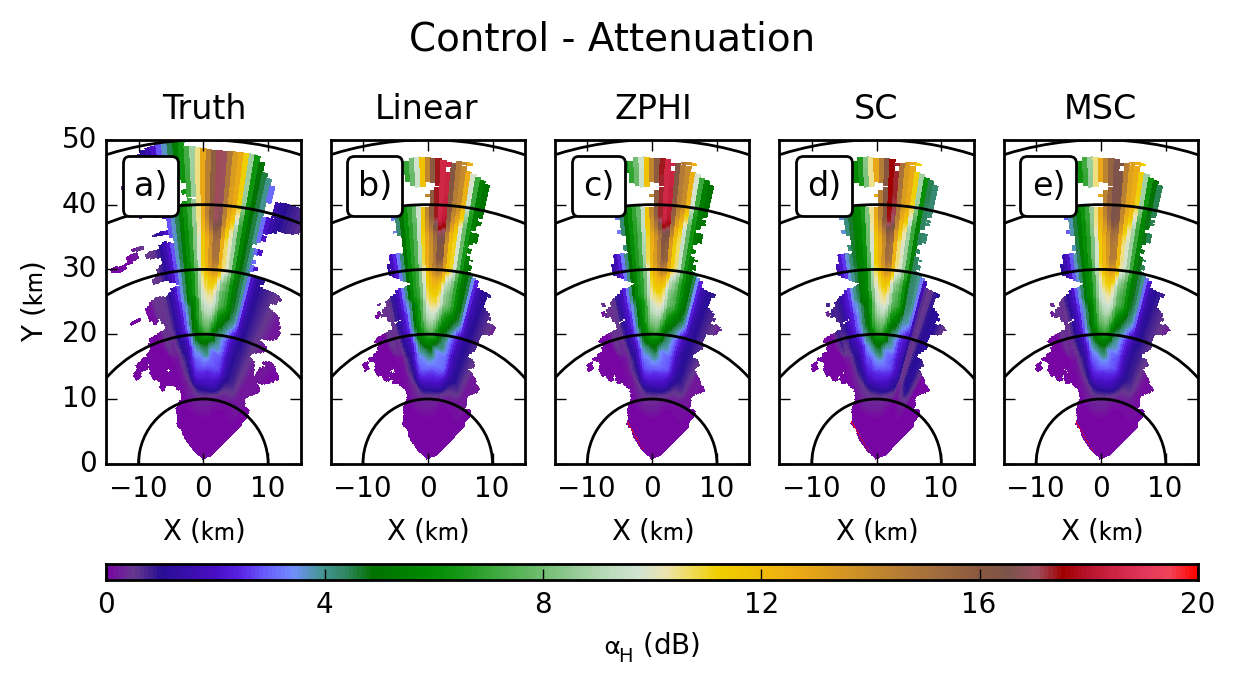
\includegraphics[scale=0.7]{figures/spatial/C_Control_Attenuation_H}
    \end{center}
\end{frame}

\begin{frame}
    \begin{center}
        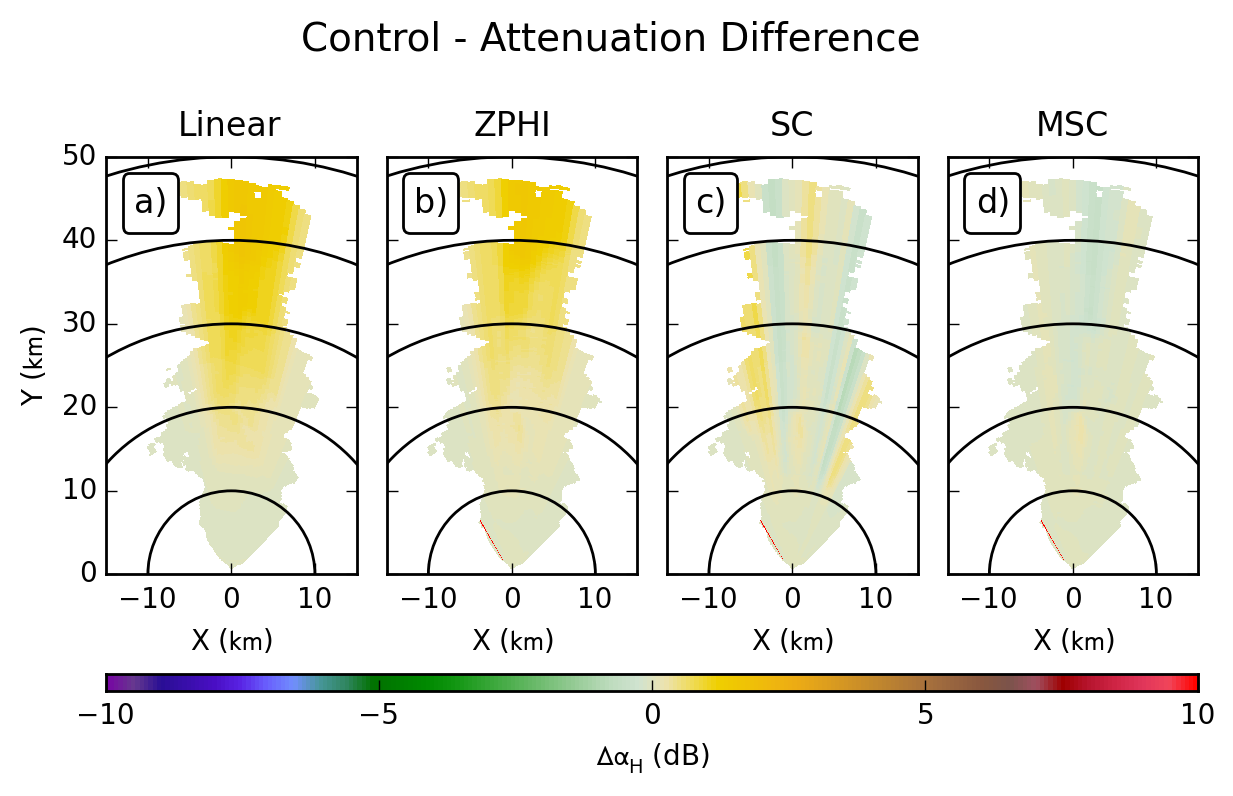
\includegraphics[scale=0.7]{figures/spatial/C_Control_Attenuation_Difference_H}
    \end{center}
\end{frame}

\begin{frame}
    \begin{center}
        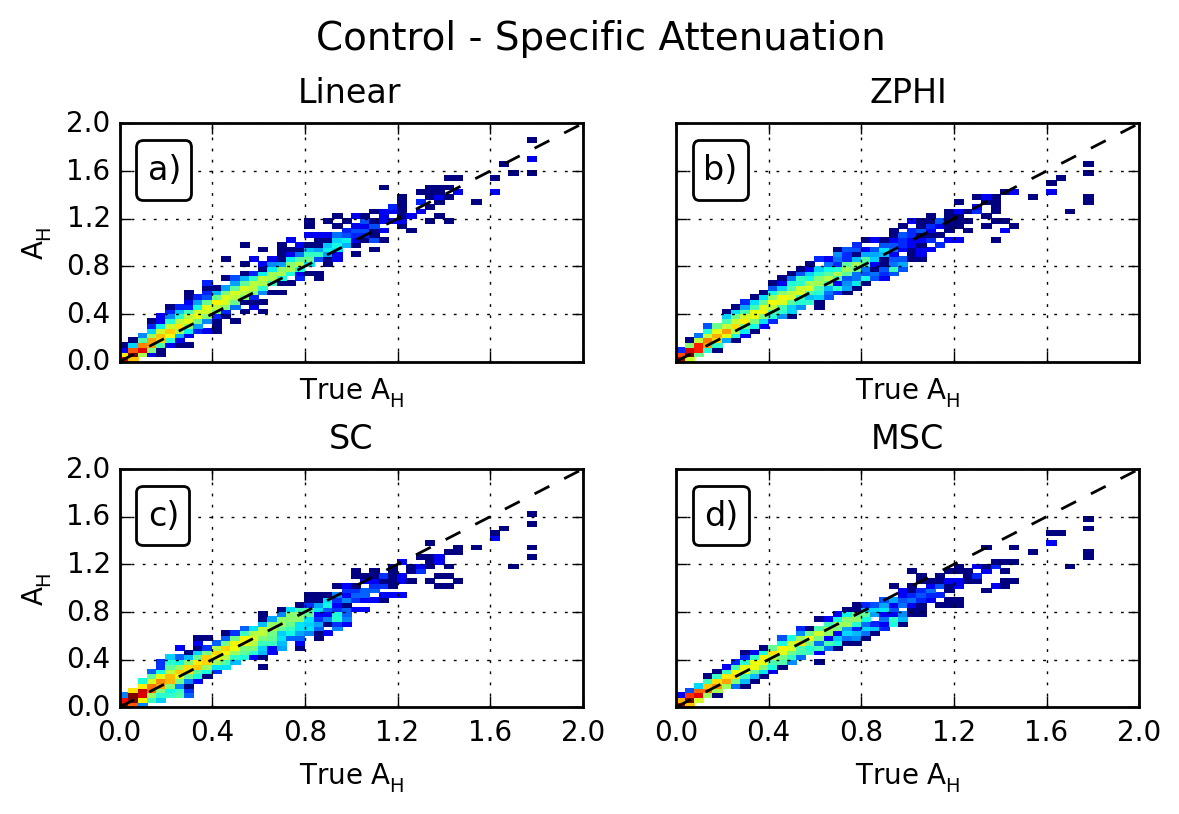
\includegraphics[scale=0.7]{figures/spatial/C_Control_Specific_Attenuation_H_scatter}
    \end{center}
\end{frame}

\begin{frame}
    \begin{center}
        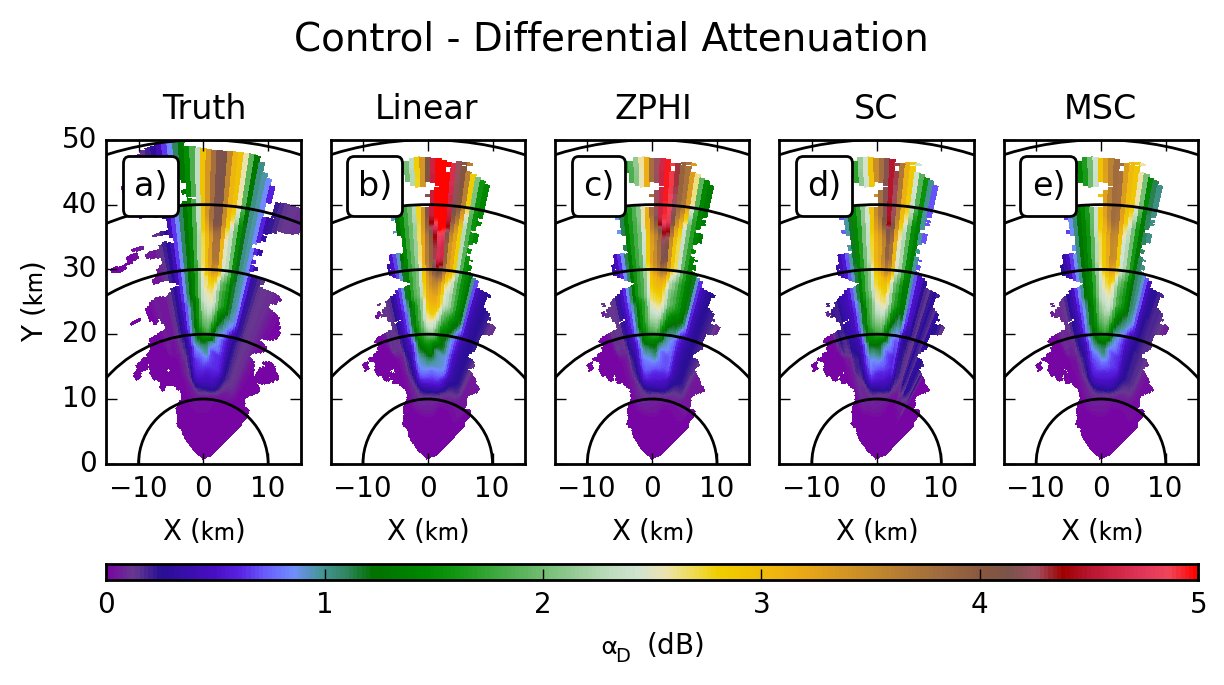
\includegraphics[scale=0.7]{figures/spatial/C_Control_Differential_Attenuation}
    \end{center}
\end{frame}

\begin{frame}
    \begin{center}
        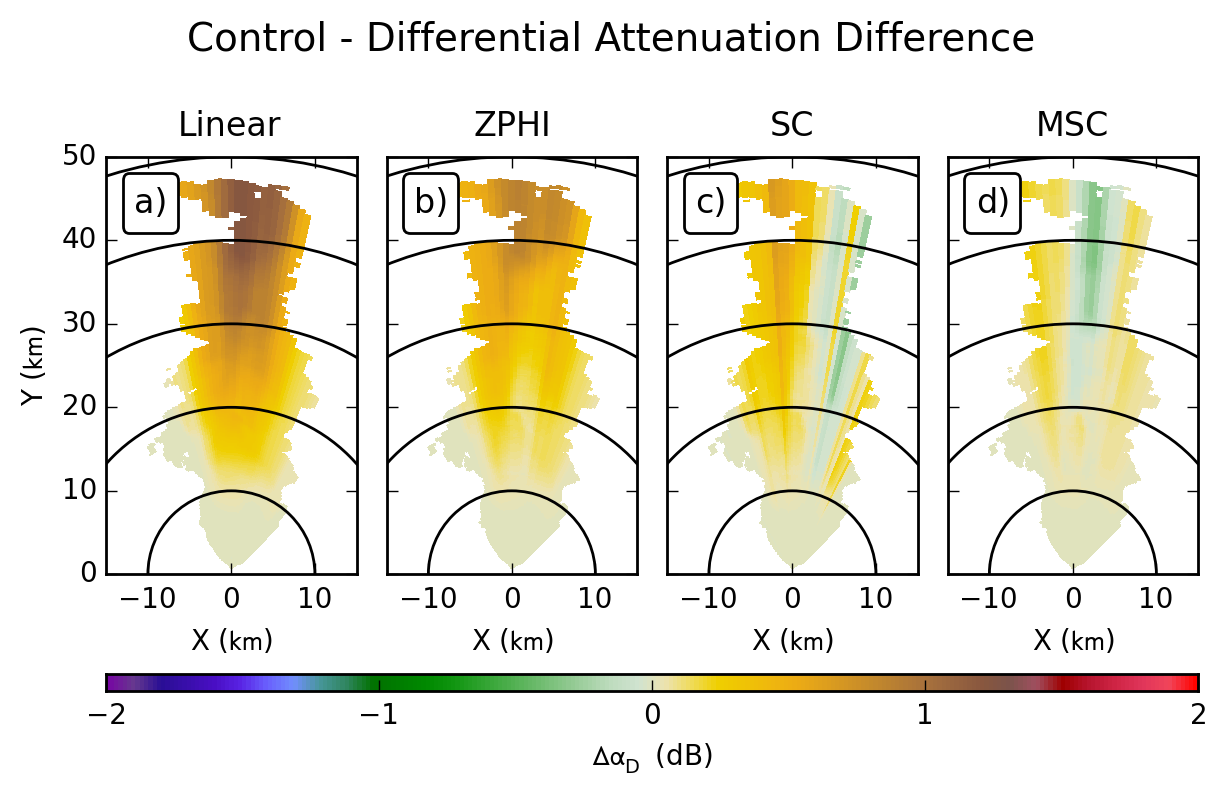
\includegraphics[scale=0.7]{figures/spatial/C_Control_Differential_Attenuation_Difference}
    \end{center}
\end{frame}

\begin{frame}
    \begin{center}
        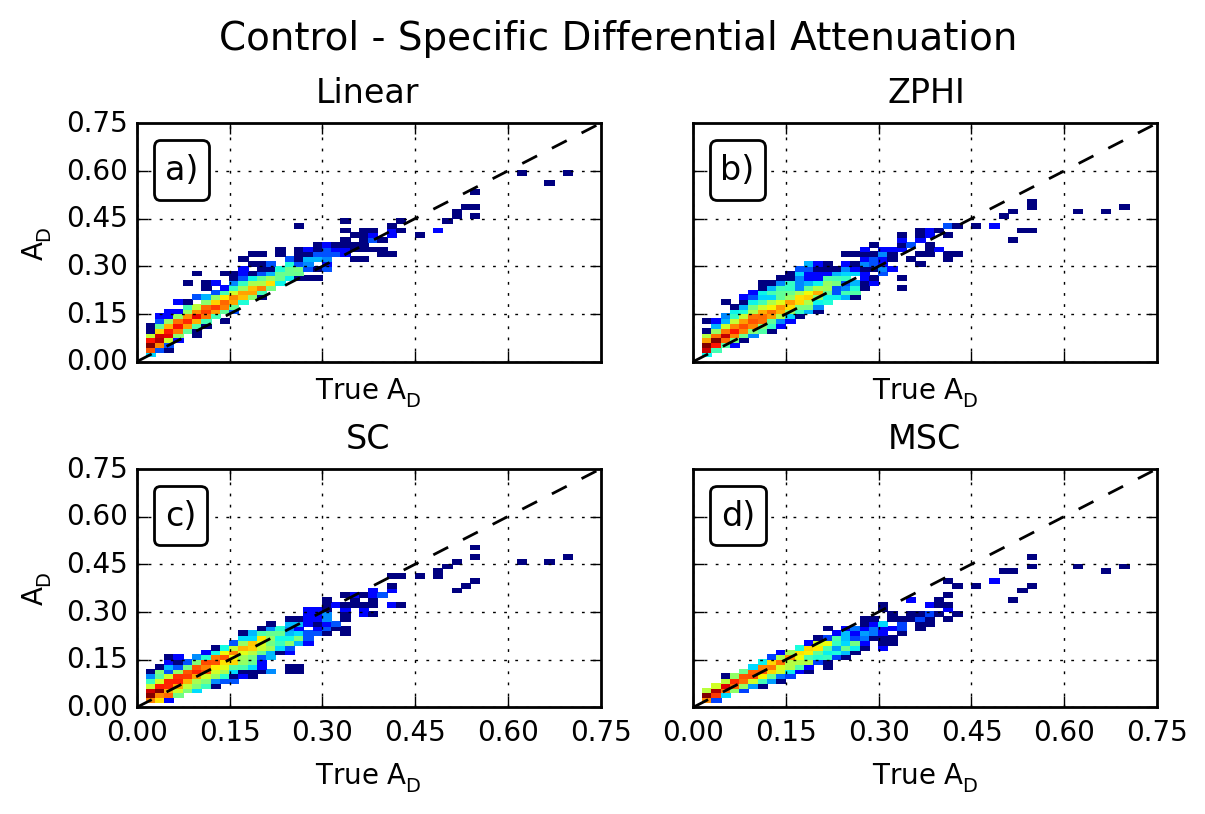
\includegraphics[scale=0.7]{figures/spatial/C_Control_Specific_Differential_Attenuation_scatter}
    \end{center}
\end{frame}

\begin{frame}
    \begin{center}
        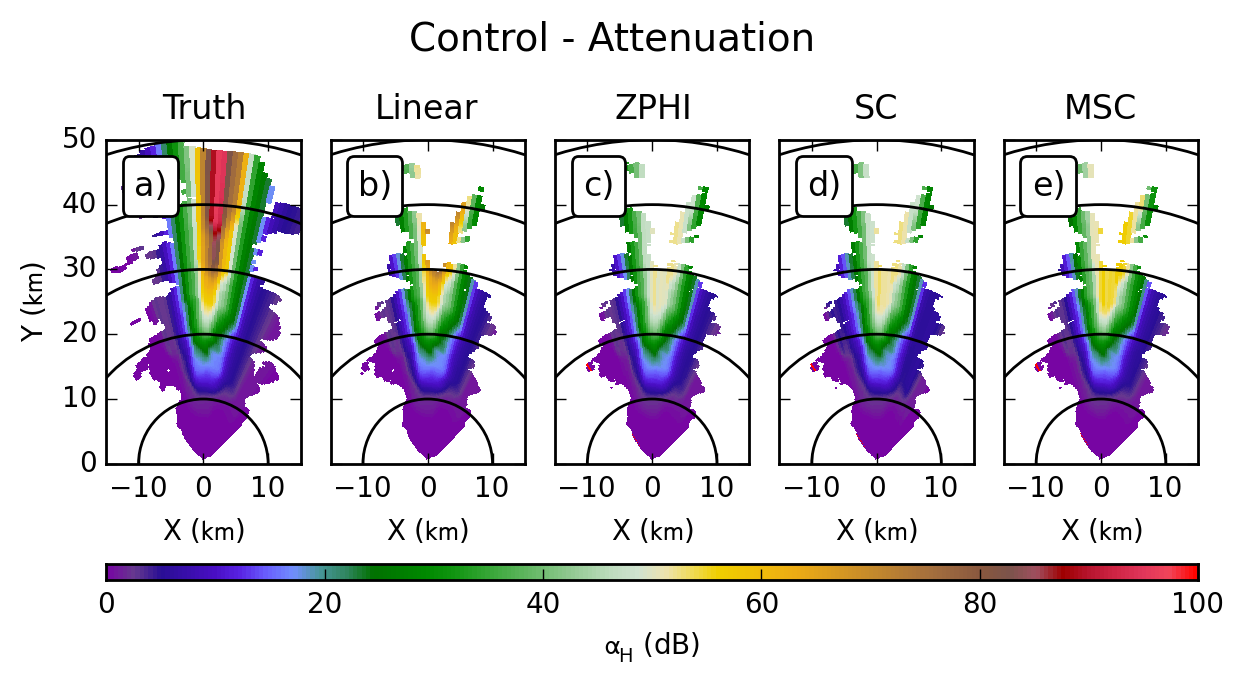
\includegraphics[scale=0.7]{figures/spatial/X_Control_Attenuation_H}
    \end{center}
\end{frame}

\begin{frame}
    \begin{center}
        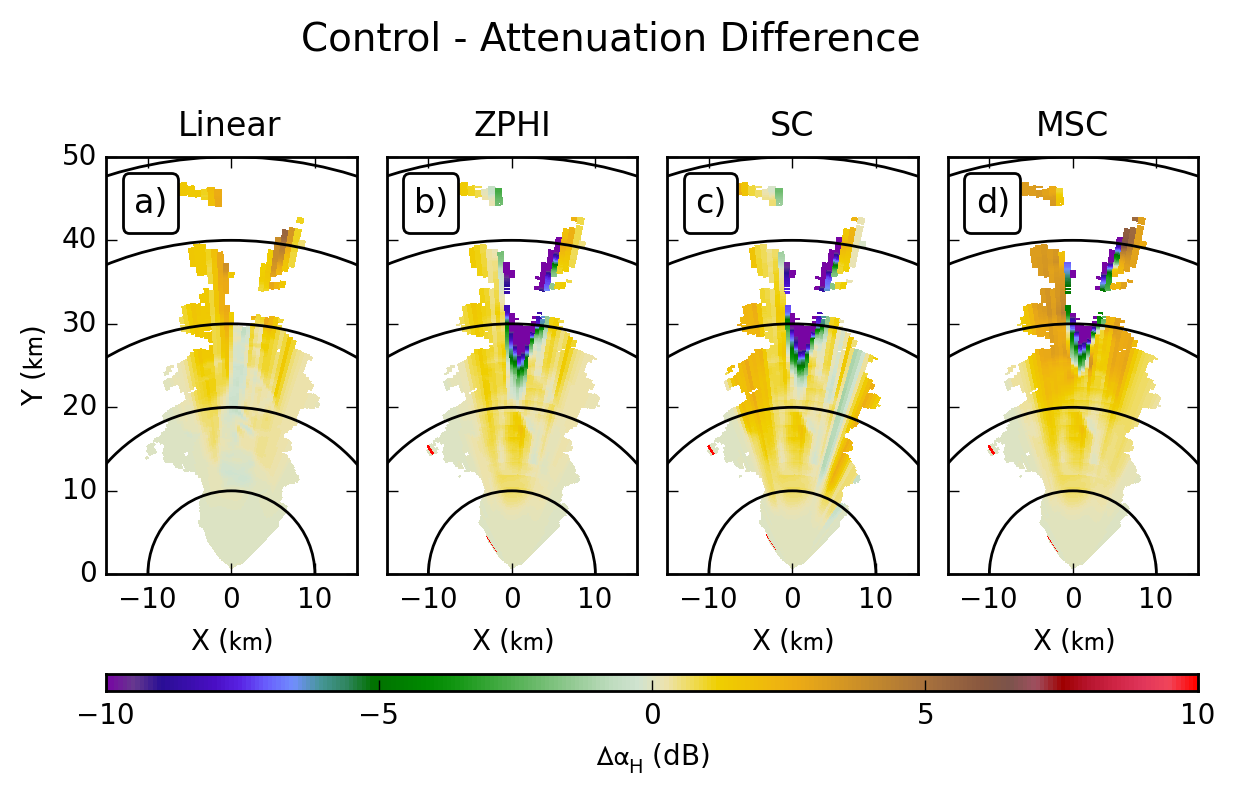
\includegraphics[scale=0.7]{figures/spatial/X_Control_Attenuation_Difference_H}
    \end{center}
\end{frame}

\begin{frame}
    \begin{center}
        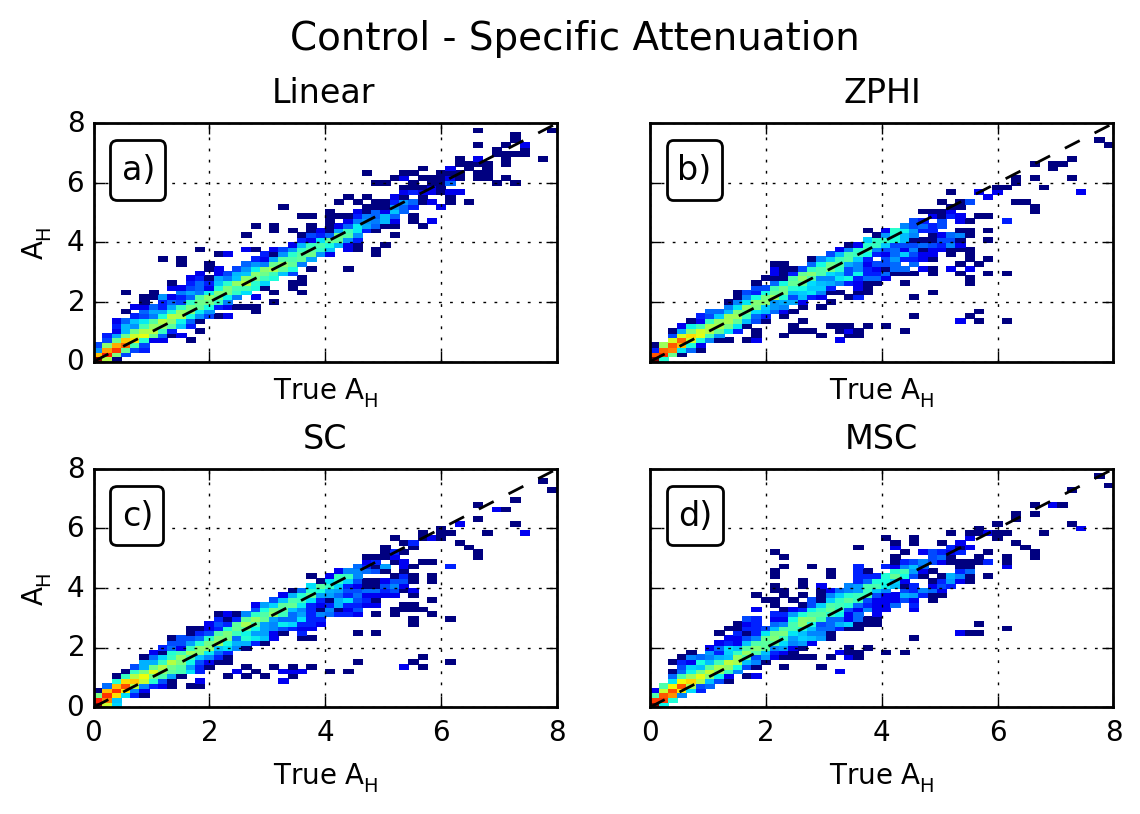
\includegraphics[scale=0.7]{figures/spatial/X_Control_Specific_Attenuation_H_scatter}
    \end{center}
\end{frame}

\begin{frame}
    \begin{center}
        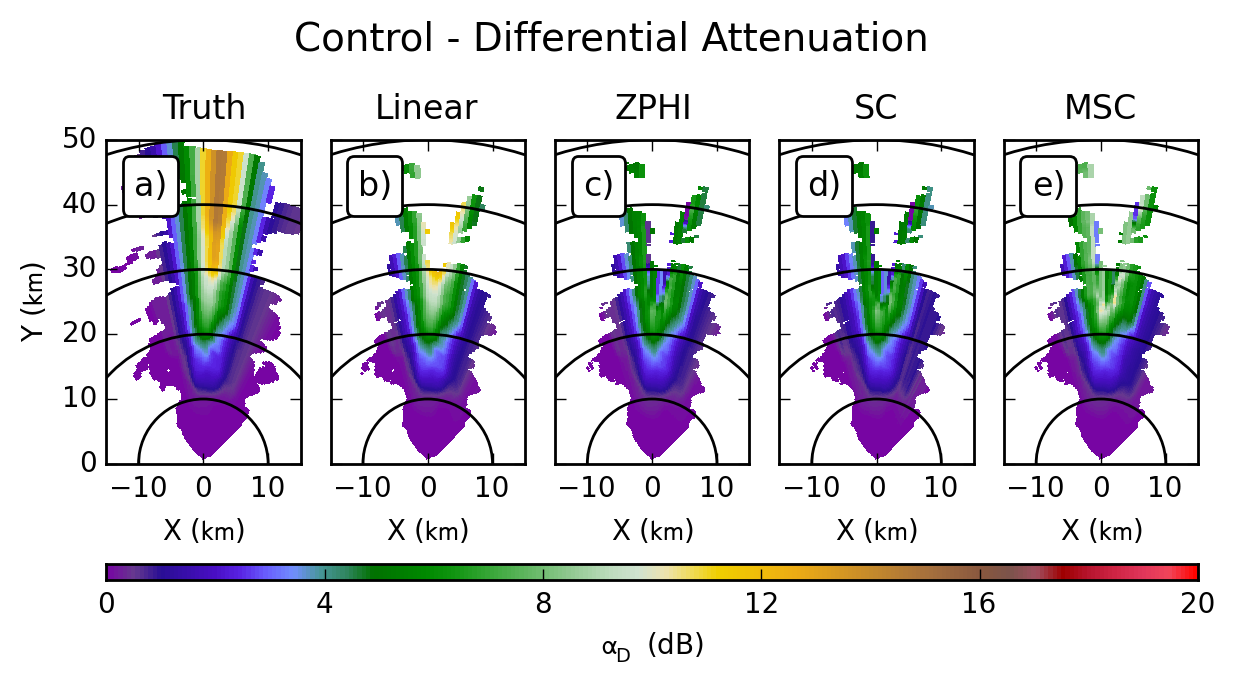
\includegraphics[scale=0.7]{figures/spatial/X_Control_Differential_Attenuation}
    \end{center}
\end{frame}

\begin{frame}
    \begin{center}
        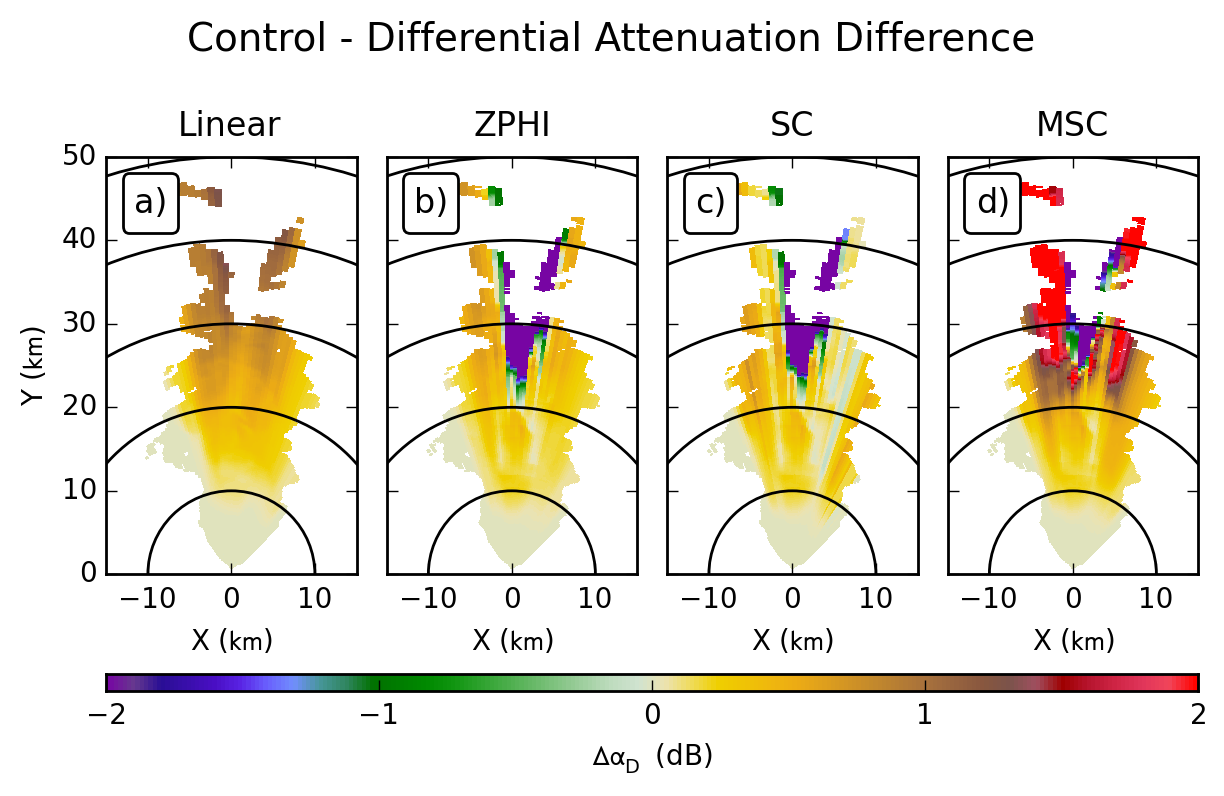
\includegraphics[scale=0.7]{figures/spatial/X_Control_Differential_Attenuation_Difference}
    \end{center}
\end{frame}

\begin{frame}
    \begin{center}
        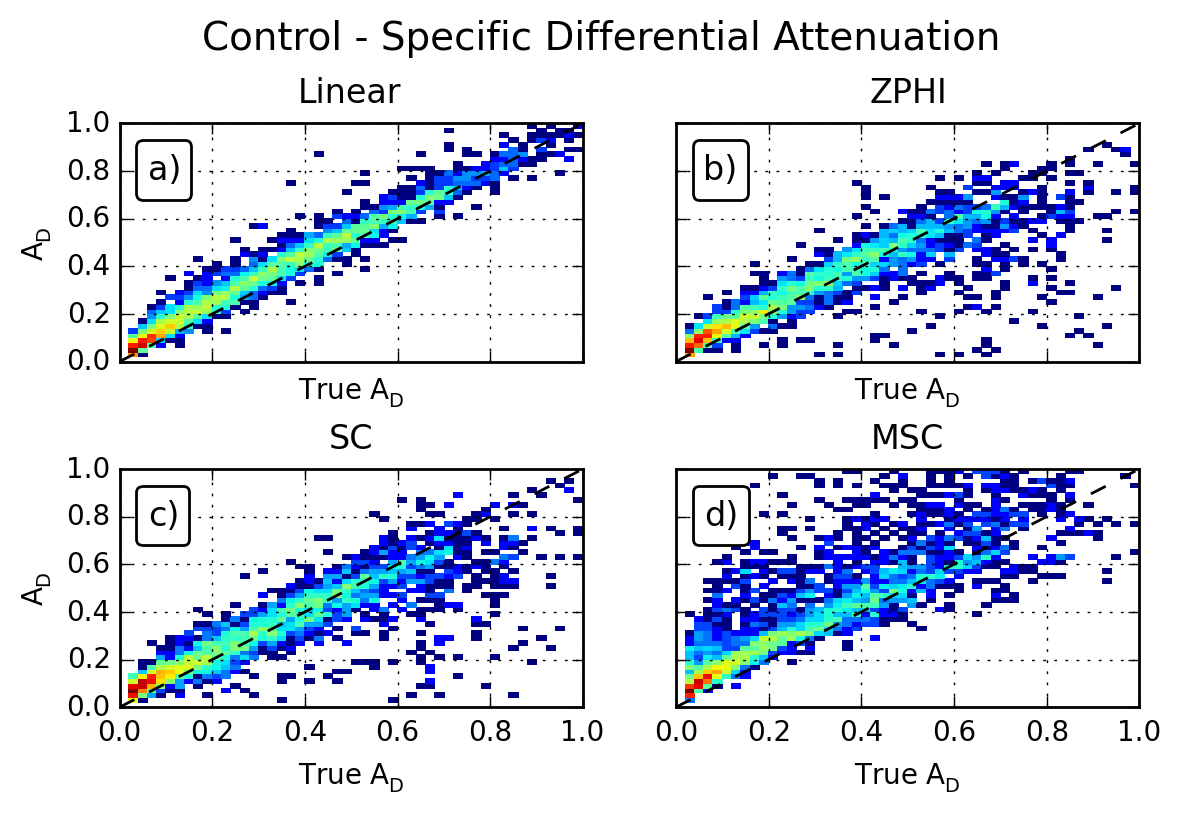
\includegraphics[scale=0.7]{figures/spatial/X_Control_Specific_Differential_Attenuation_scatter}
    \end{center}
\end{frame}

\subsubsection{Sidelobe}
\begin{frame}
    \begin{center}
        \includegraphics<1>[scale=0.7]{figures/spatial/C_Sidelobe_Attenuation_H}
        \includegraphics<2>[scale=0.7]{figures/spatial/C_Control_Attenuation_H}
    \end{center}
\end{frame}

\begin{frame}
    \begin{center}
        \includegraphics<1>[scale=0.7]{figures/spatial/C_Sidelobe_Attenuation_Difference_H}
        \includegraphics<2>[scale=0.7]{figures/spatial/C_Control_Attenuation_Difference_H}
    \end{center}
\end{frame}

\begin{frame}
    \begin{center}
        \includegraphics<1>[scale=0.7]{figures/spatial/C_Sidelobe_Specific_Attenuation_H_scatter}
        \includegraphics<2>[scale=0.7]{figures/spatial/C_Control_Specific_Attenuation_H_scatter}
    \end{center}
\end{frame}

\begin{frame}
    \begin{center}
        \includegraphics<1>[scale=0.7]{figures/spatial/C_Sidelobe_Differential_Attenuation}
        \includegraphics<2>[scale=0.7]{figures/spatial/C_Control_Differential_Attenuation}
    \end{center}
\end{frame}

\begin{frame}
    \begin{center}
        \includegraphics<1>[scale=0.7]{figures/spatial/C_Sidelobe_Differential_Attenuation_Difference}
        \includegraphics<2>[scale=0.7]{figures/spatial/C_Control_Differential_Attenuation_Difference}
    \end{center}
\end{frame}

\begin{frame}
    \begin{center}
        \includegraphics<1>[scale=0.7]{figures/spatial/C_Sidelobe_Specific_Differential_Attenuation_scatter}
        \includegraphics<2>[scale=0.7]{figures/spatial/C_Control_Specific_Differential_Attenuation_scatter}
    \end{center}
\end{frame}

\begin{frame}
    \begin{center}
        \includegraphics<1>[scale=0.7]{figures/spatial/X_Sidelobe_Attenuation_H}
        \includegraphics<2>[scale=0.7]{figures/spatial/X_Control_Attenuation_H}
    \end{center}
\end{frame}

\begin{frame}
    \begin{center}
        \includegraphics<1>[scale=0.7]{figures/spatial/X_Sidelobe_Attenuation_Difference_H}
        \includegraphics<2>[scale=0.7]{figures/spatial/X_Control_Attenuation_Difference_H}
    \end{center}
\end{frame}

\begin{frame}
    \begin{center}
        \includegraphics<1>[scale=0.7]{figures/spatial/X_Sidelobe_Specific_Attenuation_H_scatter}
        \includegraphics<2>[scale=0.7]{figures/spatial/X_Control_Specific_Attenuation_H_scatter}
    \end{center}
\end{frame}

\begin{frame}
    \begin{center}
        \includegraphics<1>[scale=0.7]{figures/spatial/X_Sidelobe_Differential_Attenuation}
        \includegraphics<2>[scale=0.7]{figures/spatial/X_Control_Differential_Attenuation}
    \end{center}
\end{frame}

\begin{frame}
    \begin{center}
        \includegraphics<1>[scale=0.7]{figures/spatial/X_Sidelobe_Differential_Attenuation_Difference}
        \includegraphics<2>[scale=0.7]{figures/spatial/X_Control_Differential_Attenuation_Difference}
    \end{center}
\end{frame}

\begin{frame}
    \begin{center}
        \includegraphics<1>[scale=0.7]{figures/spatial/X_Sidelobe_Specific_Differential_Attenuation_scatter}
        \includegraphics<2>[scale=0.7]{figures/spatial/X_Control_Specific_Differential_Attenuation_scatter}
    \end{center}
\end{frame}

\subsubsection{Beamwidth}
\begin{frame}
    \begin{center}
        \includegraphics<1>[scale=0.7]{figures/spatial/C_Beamwidth_Attenuation_H}
        \includegraphics<2>[scale=0.7]{figures/spatial/C_Control_Attenuation_H}
    \end{center}
\end{frame}

\begin{frame}
    \begin{center}
        \includegraphics<1>[scale=0.7]{figures/spatial/C_Beamwidth_Attenuation_Difference_H}
        \includegraphics<2>[scale=0.7]{figures/spatial/C_Control_Attenuation_Difference_H}
    \end{center}
\end{frame}

\begin{frame}
    \begin{center}
        \includegraphics<1>[scale=0.7]{figures/spatial/C_Beamwidth_Specific_Attenuation_H_scatter}
        \includegraphics<2>[scale=0.7]{figures/spatial/C_Control_Specific_Attenuation_H_scatter}
    \end{center}
\end{frame}

\begin{frame}
    \begin{center}
        \includegraphics<1>[scale=0.7]{figures/spatial/C_Beamwidth_Differential_Attenuation}
        \includegraphics<2>[scale=0.7]{figures/spatial/C_Control_Differential_Attenuation}
    \end{center}
\end{frame}

\begin{frame}
    \begin{center}
        \includegraphics<1>[scale=0.7]{figures/spatial/C_Beamwidth_Differential_Attenuation_Difference}
        \includegraphics<2>[scale=0.7]{figures/spatial/C_Control_Differential_Attenuation_Difference}
    \end{center}
\end{frame}

\begin{frame}
    \begin{center}
        \includegraphics<1>[scale=0.7]{figures/spatial/C_Beamwidth_Specific_Differential_Attenuation_scatter}
        \includegraphics<2>[scale=0.7]{figures/spatial/C_Control_Specific_Differential_Attenuation_scatter}
    \end{center}
\end{frame}

\begin{frame}
    \begin{center}
        \includegraphics<1>[scale=0.7]{figures/spatial/X_Beamwidth_Attenuation_H}
        \includegraphics<2>[scale=0.7]{figures/spatial/X_Control_Attenuation_H}
    \end{center}
\end{frame}

\begin{frame}
    \begin{center}
        \includegraphics<1>[scale=0.7]{figures/spatial/X_Beamwidth_Attenuation_Difference_H}
        \includegraphics<2>[scale=0.7]{figures/spatial/X_Control_Attenuation_Difference_H}
    \end{center}
\end{frame}

\begin{frame}
    \begin{center}
        \includegraphics<1>[scale=0.7]{figures/spatial/X_Beamwidth_Specific_Attenuation_H_scatter}
        \includegraphics<2>[scale=0.7]{figures/spatial/X_Control_Specific_Attenuation_H_scatter}
    \end{center}
\end{frame}

\begin{frame}
    \begin{center}
        \includegraphics<1>[scale=0.7]{figures/spatial/X_Beamwidth_Differential_Attenuation}
        \includegraphics<2>[scale=0.7]{figures/spatial/X_Control_Differential_Attenuation}
    \end{center}
\end{frame}

\begin{frame}
    \begin{center}
        \includegraphics<1>[scale=0.7]{figures/spatial/X_Beamwidth_Differential_Attenuation_Difference}
        \includegraphics<2>[scale=0.7]{figures/spatial/X_Control_Differential_Attenuation_Difference}
    \end{center}
\end{frame}

\begin{frame}
    \begin{center}
        \includegraphics<1>[scale=0.7]{figures/spatial/X_Beamwidth_Specific_Differential_Attenuation_scatter}
        \includegraphics<2>[scale=0.7]{figures/spatial/X_Control_Specific_Differential_Attenuation_scatter}
    \end{center}
\end{frame}

\subsubsection{Range Resolution}
\begin{frame}
    \begin{center}
        \includegraphics<1>[scale=0.7]{figures/spatial/C_RangeResolution_Attenuation_H}
        \includegraphics<2>[scale=0.7]{figures/spatial/C_Control_Attenuation_H}
    \end{center}
\end{frame}

\begin{frame}
    \begin{center}
        \includegraphics<1>[scale=0.7]{figures/spatial/C_RangeResolution_Differential_Attenuation}
        \includegraphics<2>[scale=0.7]{figures/spatial/C_Control_Differential_Attenuation}
    \end{center}
\end{frame}

\begin{frame}
    \begin{center}
        \includegraphics<1>[scale=0.7]{figures/spatial/X_RangeResolution_Attenuation_H}
        \includegraphics<2>[scale=0.7]{figures/spatial/X_Control_Attenuation_H}
    \end{center}
\end{frame}

\begin{frame}
    \begin{center}
        \includegraphics<1>[scale=0.7]{figures/spatial/X_RangeResolution_Attenuation_Difference_H}
        \includegraphics<2>[scale=0.7]{figures/spatial/X_Control_Attenuation_Difference_H}
    \end{center}
\end{frame}

\begin{frame}
    \begin{center}
        \includegraphics<1>[scale=0.7]{figures/spatial/X_RangeResolution_Specific_Attenuation_H_scatter}
        \includegraphics<2>[scale=0.7]{figures/spatial/X_Control_Specific_Attenuation_H_scatter}
    \end{center}
\end{frame}

\begin{frame}
    \begin{center}
        \includegraphics<1>[scale=0.7]{figures/spatial/X_RangeResolution_Differential_Attenuation}
        \includegraphics<2>[scale=0.7]{figures/spatial/X_Control_Differential_Attenuation}
    \end{center}
\end{frame}

\begin{frame}
    \begin{center}
        \includegraphics<1>[scale=0.7]{figures/spatial/X_RangeResolution_Differential_Attenuation_Difference}
        \includegraphics<2>[scale=0.7]{figures/spatial/X_Control_Differential_Attenuation_Difference}
    \end{center}
\end{frame}

\begin{frame}
    \begin{center}
        \includegraphics<1>[scale=0.7]{figures/spatial/X_RangeResolution_Specific_Differential_Attenuation_scatter}
        \includegraphics<2>[scale=0.7]{figures/spatial/X_Control_Specific_Differential_Attenuation_scatter}
    \end{center}
\end{frame}

\subsubsection{Radial Width}
\begin{frame}
    \begin{center}
        \includegraphics<1>[scale=0.7]{figures/spatial/C_RadialWidth_Attenuation_H}
        \includegraphics<2>[scale=0.7]{figures/spatial/C_Control_Attenuation_H}
    \end{center}
\end{frame}

\begin{frame}
    \begin{center}
        \includegraphics<1>[scale=0.7]{figures/spatial/C_RadialWidth_Differential_Attenuation}
        \includegraphics<2>[scale=0.7]{figures/spatial/C_Control_Differential_Attenuation}
    \end{center}
\end{frame}

\begin{frame}
    \begin{center}
        \includegraphics<1>[scale=0.7]{figures/spatial/X_RadialWidth_Attenuation_H}
        \includegraphics<2>[scale=0.7]{figures/spatial/X_Control_Attenuation_H}
    \end{center}
\end{frame}

\begin{frame}
    \begin{center}
        \includegraphics<1>[scale=0.7]{figures/spatial/X_RadialWidth_Attenuation_Difference_H}
        \includegraphics<2>[scale=0.7]{figures/spatial/X_Control_Attenuation_Difference_H}
    \end{center}
\end{frame}

\begin{frame}
    \begin{center}
        \includegraphics<1>[scale=0.7]{figures/spatial/X_RadialWidth_Specific_Attenuation_H_scatter}
        \includegraphics<2>[scale=0.7]{figures/spatial/X_Control_Specific_Attenuation_H_scatter}
    \end{center}
\end{frame}

\begin{frame}
    \begin{center}
        \includegraphics<1>[scale=0.7]{figures/spatial/X_RadialWidth_Differential_Attenuation}
        \includegraphics<2>[scale=0.7]{figures/spatial/X_Control_Differential_Attenuation}
    \end{center}
\end{frame}

\begin{frame}
    \begin{center}
        \includegraphics<1>[scale=0.7]{figures/spatial/X_RadialWidth_Differential_Attenuation_Difference}
        \includegraphics<2>[scale=0.7]{figures/spatial/X_Control_Differential_Attenuation_Difference}
    \end{center}
\end{frame}

\begin{frame}
    \begin{center}
        \includegraphics<1>[scale=0.7]{figures/spatial/X_RadialWidth_Specific_Differential_Attenuation_scatter}
        \includegraphics<2>[scale=0.7]{figures/spatial/X_Control_Specific_Differential_Attenuation_scatter}
    \end{center}
\end{frame}

\subsubsection{Vertical Channel}
\begin{frame}
    \begin{center}
        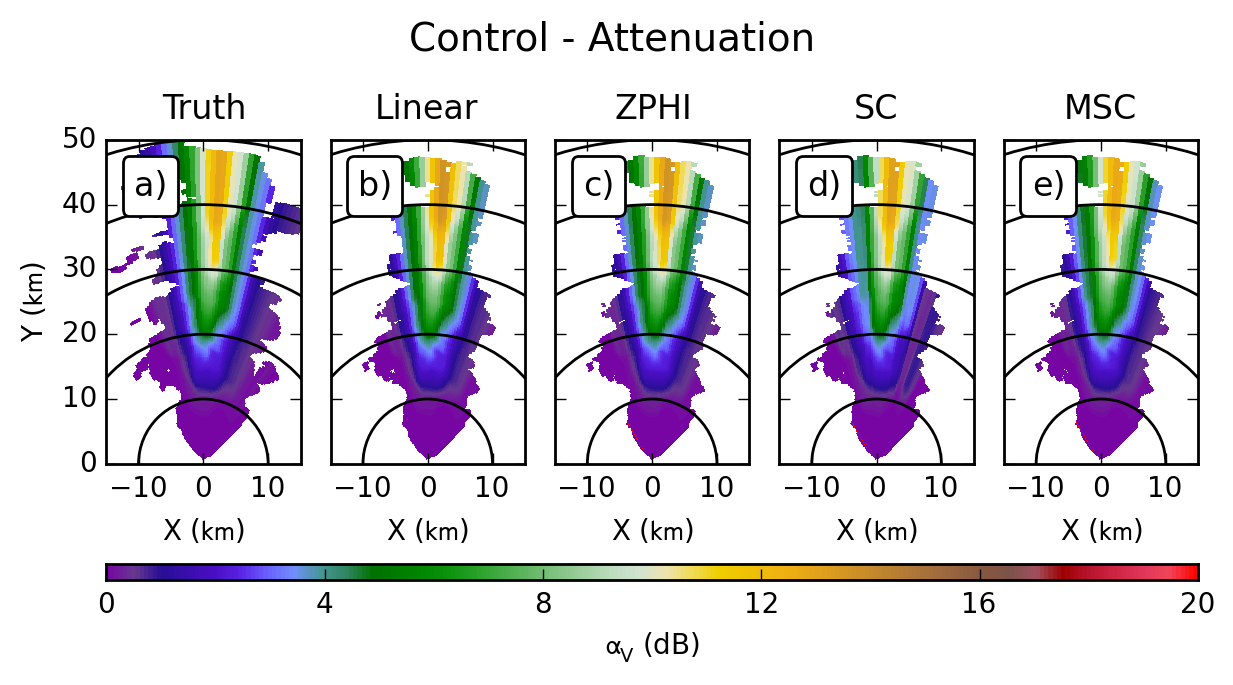
\includegraphics[scale=0.7]{figures/spatial/C_Control_Attenuation_V}
    \end{center}
\end{frame}

\begin{frame}
    \begin{center}
        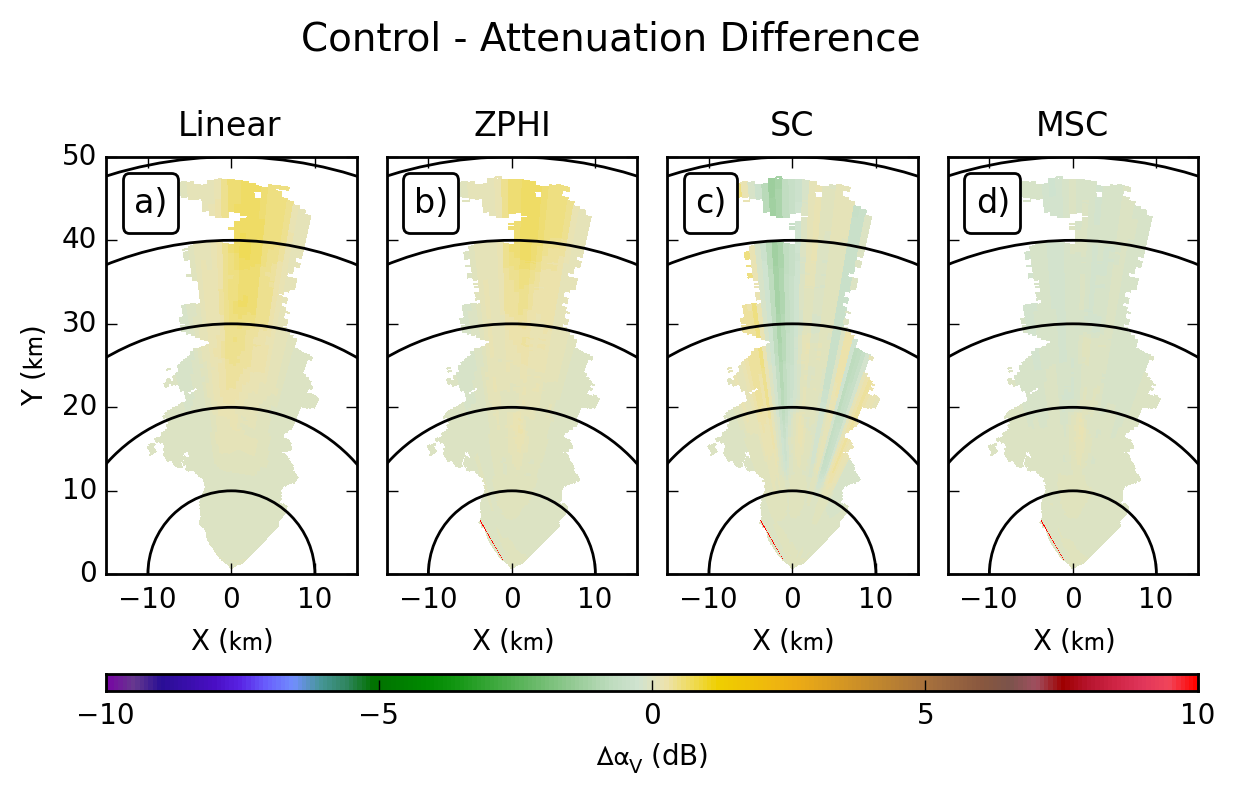
\includegraphics[scale=0.7]{figures/spatial/C_Control_Attenuation_Difference_V}
    \end{center}
\end{frame}

\begin{frame}
    \begin{center}
        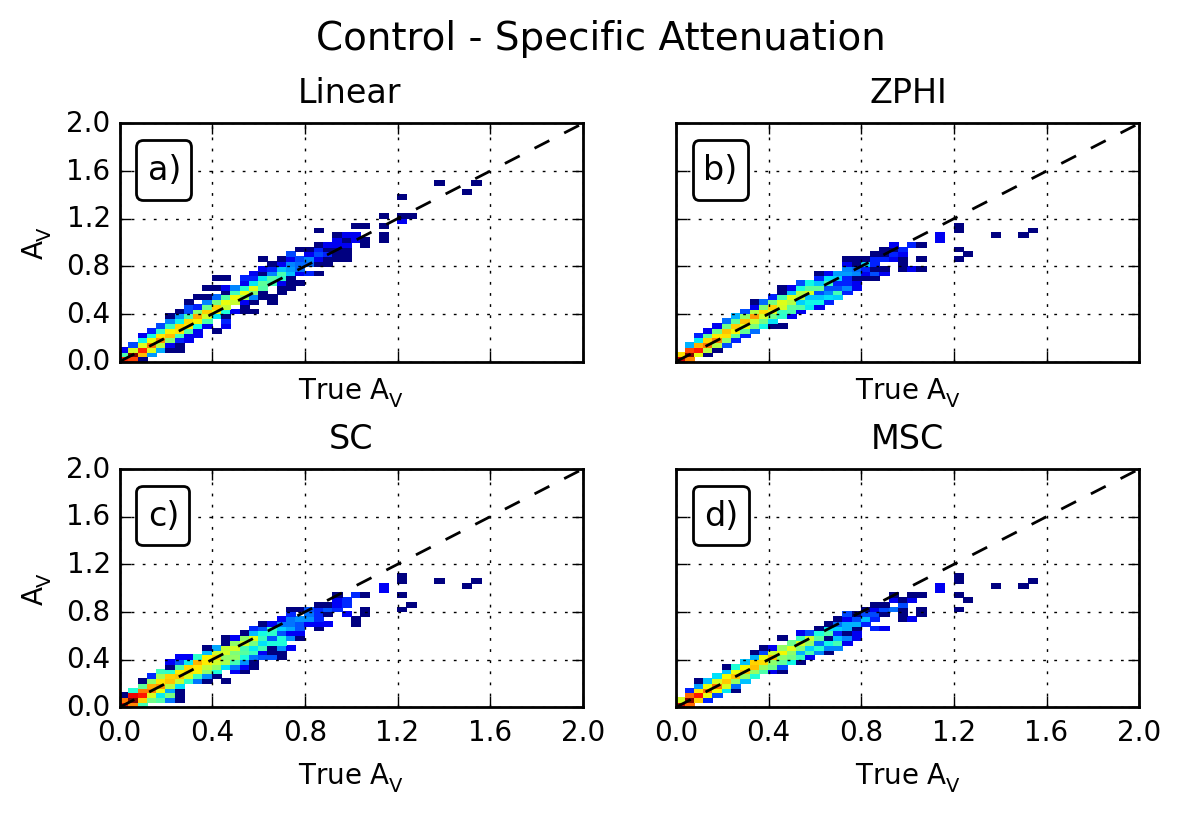
\includegraphics[scale=0.7]{figures/spatial/C_Control_Specific_Attenuation_V_scatter}
    \end{center}
\end{frame}

\begin{frame}
    \begin{center}
        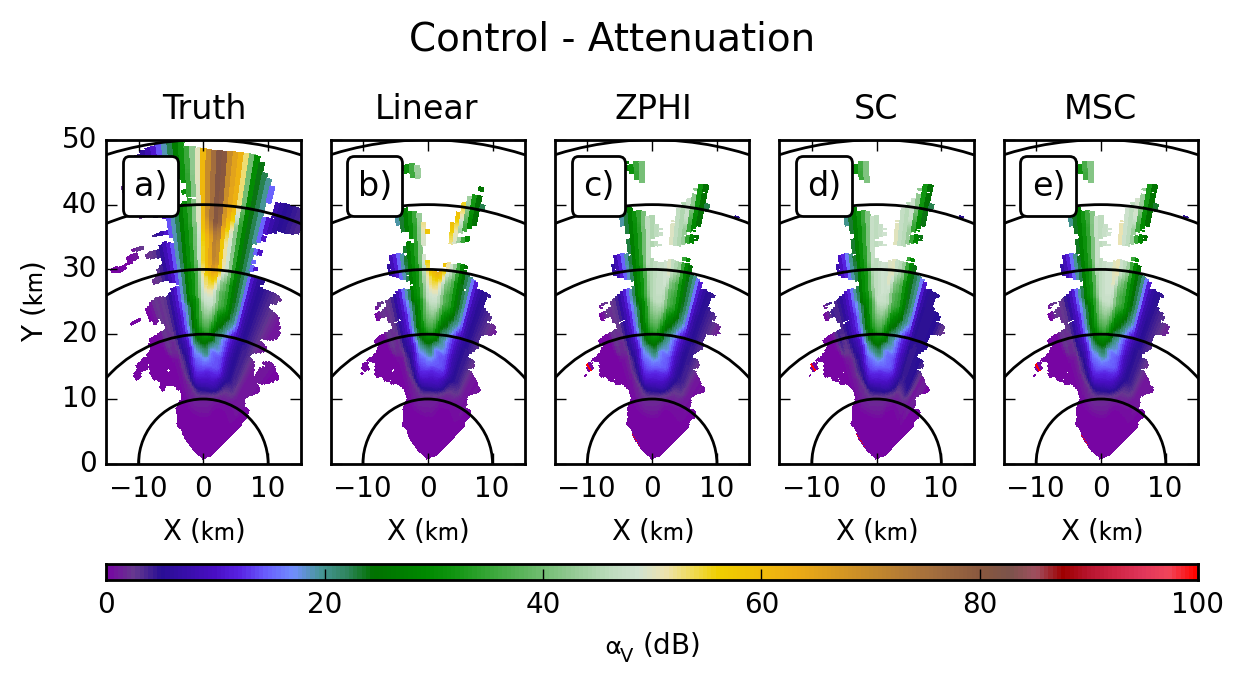
\includegraphics[scale=0.7]{figures/spatial/X_Control_Attenuation_V}
    \end{center}
\end{frame}

\begin{frame}
    \begin{center}
        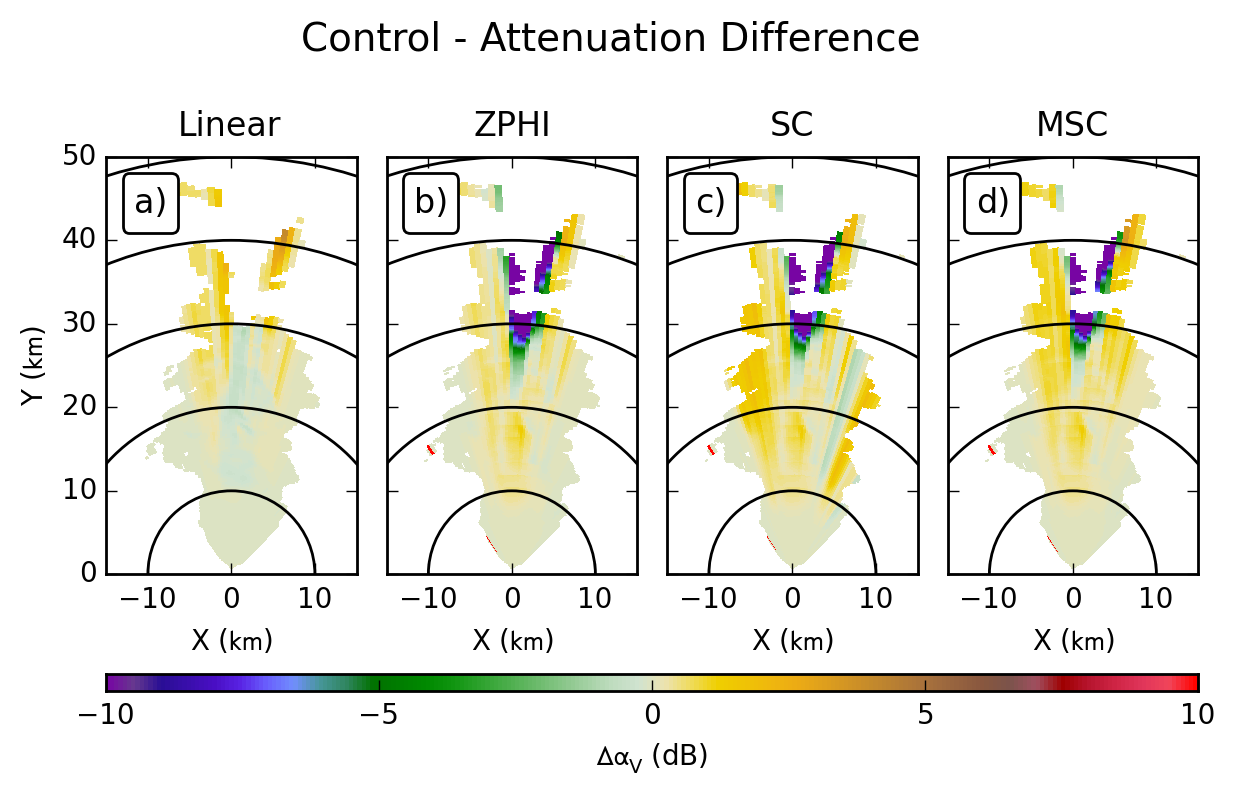
\includegraphics[scale=0.7]{figures/spatial/X_Control_Attenuation_Difference_V}
    \end{center}
\end{frame}

\begin{frame}
    \begin{center}
        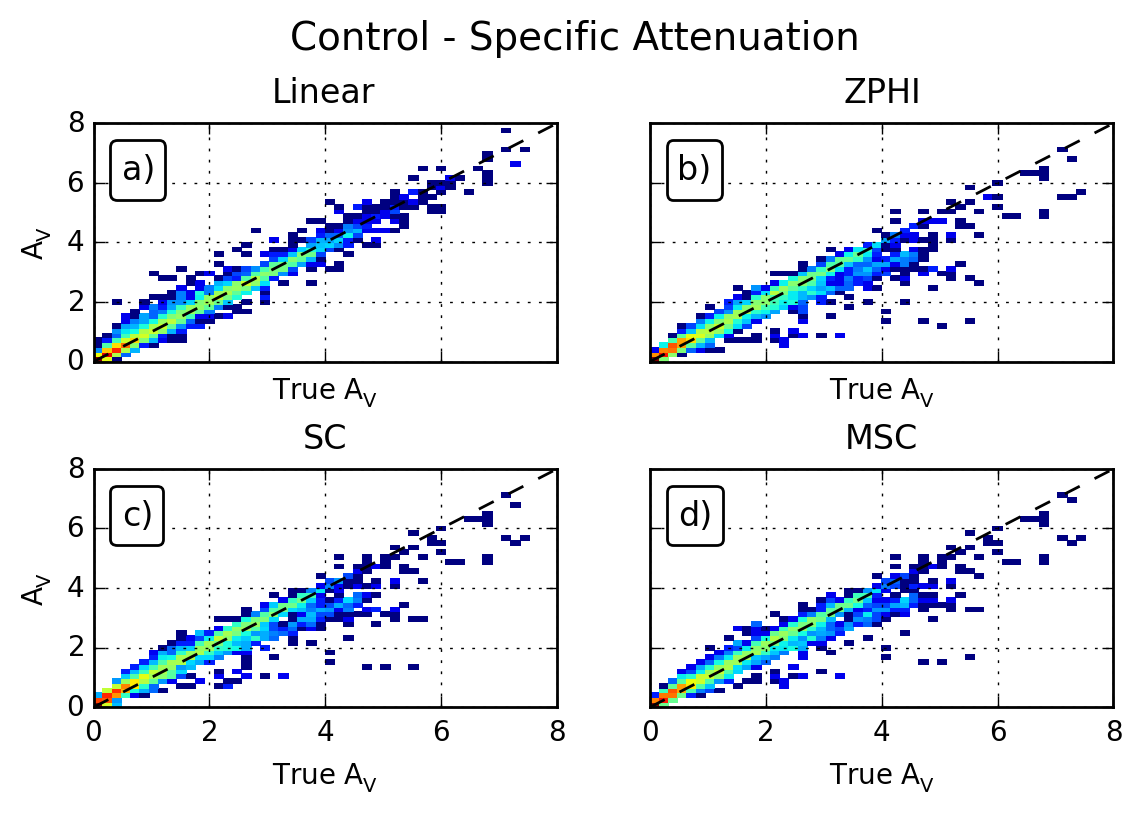
\includegraphics[scale=0.7]{figures/spatial/X_Control_Specific_Attenuation_V_scatter}
    \end{center}
\end{frame}

\begin{frame}
    \begin{center}
        \includegraphics<1>[scale=0.7]{figures/spatial/C_Sidelobe_Attenuation_V}
        \includegraphics<2>[scale=0.7]{figures/spatial/C_Control_Attenuation_V}
    \end{center}
\end{frame}

\begin{frame}
    \begin{center}
        \includegraphics<1>[scale=0.7]{figures/spatial/C_Sidelobe_Attenuation_Difference_V}
        \includegraphics<2>[scale=0.7]{figures/spatial/C_Control_Attenuation_Difference_V}
    \end{center}
\end{frame}

\begin{frame}
    \begin{center}
        \includegraphics<1>[scale=0.7]{figures/spatial/C_Sidelobe_Specific_Attenuation_V_scatter}
        \includegraphics<2>[scale=0.7]{figures/spatial/C_Control_Specific_Attenuation_V_scatter}
    \end{center}
\end{frame}

\begin{frame}
    \begin{center}
        \includegraphics<1>[scale=0.7]{figures/spatial/X_Sidelobe_Attenuation_V}
        \includegraphics<2>[scale=0.7]{figures/spatial/X_Control_Attenuation_V}
    \end{center}
\end{frame}

\begin{frame}
    \begin{center}
        \includegraphics<1>[scale=0.7]{figures/spatial/X_Sidelobe_Attenuation_Difference_V}
        \includegraphics<2>[scale=0.7]{figures/spatial/X_Control_Attenuation_Difference_V}
    \end{center}
\end{frame}

\begin{frame}
    \begin{center}
        \includegraphics<1>[scale=0.7]{figures/spatial/X_Sidelobe_Specific_Attenuation_V_scatter}
        \includegraphics<2>[scale=0.7]{figures/spatial/X_Control_Specific_Attenuation_V_scatter}
    \end{center}
\end{frame}

\begin{frame}
    \begin{center}
        \includegraphics<1>[scale=0.7]{figures/spatial/C_Beamwidth_Attenuation_V}
        \includegraphics<2>[scale=0.7]{figures/spatial/C_Control_Attenuation_V}
    \end{center}
\end{frame}

\begin{frame}
    \begin{center}
        \includegraphics<1>[scale=0.7]{figures/spatial/C_Beamwidth_Attenuation_Difference_V}
        \includegraphics<2>[scale=0.7]{figures/spatial/C_Control_Attenuation_Difference_V}
    \end{center}
\end{frame}

\begin{frame}
    \begin{center}
        \includegraphics<1>[scale=0.7]{figures/spatial/C_Beamwidth_Specific_Attenuation_V_scatter}
        \includegraphics<2>[scale=0.7]{figures/spatial/C_Control_Specific_Attenuation_V_scatter}
    \end{center}
\end{frame}

\begin{frame}
    \begin{center}
        \includegraphics<1>[scale=0.7]{figures/spatial/X_Beamwidth_Attenuation_V}
        \includegraphics<2>[scale=0.7]{figures/spatial/X_Control_Attenuation_V}
    \end{center}
\end{frame}

\begin{frame}
    \begin{center}
        \includegraphics<1>[scale=0.7]{figures/spatial/X_Beamwidth_Attenuation_Difference_V}
        \includegraphics<2>[scale=0.7]{figures/spatial/X_Control_Attenuation_Difference_V}
    \end{center}
\end{frame}

\begin{frame}
    \begin{center}
        \includegraphics<1>[scale=0.7]{figures/spatial/X_Beamwidth_Specific_Attenuation_V_scatter}
        \includegraphics<2>[scale=0.7]{figures/spatial/X_Control_Specific_Attenuation_V_scatter}
    \end{center}
\end{frame}

\begin{frame}
    \begin{center}
        \includegraphics<1>[scale=0.7]{figures/spatial/C_RadialWidth_Attenuation_V}
        \includegraphics<2>[scale=0.7]{figures/spatial/C_Control_Attenuation_V}
    \end{center}
\end{frame}

\begin{frame}
    \begin{center}
        \includegraphics<1>[scale=0.7]{figures/spatial/C_RadialWidth_Attenuation_Difference_V}
        \includegraphics<2>[scale=0.7]{figures/spatial/C_Control_Attenuation_Difference_V}
    \end{center}
\end{frame}

\begin{frame}
    \begin{center}
        \includegraphics<1>[scale=0.7]{figures/spatial/C_RadialWidth_Specific_Attenuation_V_scatter}
        \includegraphics<2>[scale=0.7]{figures/spatial/C_Control_Specific_Attenuation_V_scatter}
    \end{center}
\end{frame}

\begin{frame}
    \begin{center}
        \includegraphics<1>[scale=0.7]{figures/spatial/X_RadialWidth_Attenuation_V}
        \includegraphics<2>[scale=0.7]{figures/spatial/X_Control_Attenuation_V}
    \end{center}
\end{frame}

\begin{frame}
    \begin{center}
        \includegraphics<1>[scale=0.7]{figures/spatial/X_RadialWidth_Attenuation_Difference_V}
        \includegraphics<2>[scale=0.7]{figures/spatial/X_Control_Attenuation_Difference_V}
    \end{center}
\end{frame}

\begin{frame}
    \begin{center}
        \includegraphics<1>[scale=0.7]{figures/spatial/X_RadialWidth_Specific_Attenuation_V_scatter}
        \includegraphics<2>[scale=0.7]{figures/spatial/X_Control_Specific_Attenuation_V_scatter}
    \end{center}
\end{frame}

\begin{frame}
    \begin{center}
        \includegraphics<1>[scale=0.7]{figures/spatial/C_RangeResolution_Attenuation_V}
        \includegraphics<2>[scale=0.7]{figures/spatial/C_Control_Attenuation_V}
    \end{center}
\end{frame}

\begin{frame}
    \begin{center}
        \includegraphics<1>[scale=0.7]{figures/spatial/C_RangeResolution_Attenuation_Difference_V}
        \includegraphics<2>[scale=0.7]{figures/spatial/C_Control_Attenuation_Difference_V}
    \end{center}
\end{frame}

\begin{frame}
    \begin{center}
        \includegraphics<1>[scale=0.7]{figures/spatial/C_RangeResolution_Specific_Attenuation_V_scatter}
        \includegraphics<2>[scale=0.7]{figures/spatial/C_Control_Specific_Attenuation_V_scatter}
    \end{center}
\end{frame}

\begin{frame}
    \begin{center}
        \includegraphics<1>[scale=0.7]{figures/spatial/X_RangeResolution_Attenuation_V}
        \includegraphics<2>[scale=0.7]{figures/spatial/X_Control_Attenuation_V}
    \end{center}
\end{frame}

\begin{frame}
    \begin{center}
        \includegraphics<1>[scale=0.7]{figures/spatial/X_RangeResolution_Attenuation_Difference_V}
        \includegraphics<2>[scale=0.7]{figures/spatial/X_Control_Attenuation_Difference_V}
    \end{center}
\end{frame}

\begin{frame}
    \begin{center}
        \includegraphics<1>[scale=0.7]{figures/spatial/X_RangeResolution_Specific_Attenuation_V_scatter}
        \includegraphics<2>[scale=0.7]{figures/spatial/X_Control_Specific_Attenuation_V_scatter}
    \end{center}
\end{frame}

\begin{frame}
    \begin{center}
        \includegraphics<1>[scale=0.7]{figures/spatial/C_Combined_Attenuation_V}
        \includegraphics<2>[scale=0.7]{figures/spatial/C_Control_Attenuation_V}
    \end{center}
\end{frame}

\begin{frame}
    \begin{center}
        \includegraphics<1>[scale=0.7]{figures/spatial/C_Combined_Attenuation_Difference_V}
        \includegraphics<2>[scale=0.7]{figures/spatial/C_Control_Attenuation_Difference_V}
    \end{center}
\end{frame}

\begin{frame}
    \begin{center}
        \includegraphics<1>[scale=0.7]{figures/spatial/C_Combined_Specific_Attenuation_V_scatter}
        \includegraphics<2>[scale=0.7]{figures/spatial/C_Control_Specific_Attenuation_V_scatter}
    \end{center}
\end{frame}

\begin{frame}
    \begin{center}
        \includegraphics<1>[scale=0.7]{figures/spatial/X_Combined_Attenuation_V}
        \includegraphics<2>[scale=0.7]{figures/spatial/X_Control_Attenuation_V}
    \end{center}
\end{frame}

\begin{frame}
    \begin{center}
        \includegraphics<1>[scale=0.7]{figures/spatial/X_Combined_Attenuation_Difference_V}
        \includegraphics<2>[scale=0.7]{figures/spatial/X_Control_Attenuation_Difference_V}
    \end{center}
\end{frame}

\begin{frame}
    \begin{center}
        \includegraphics<1>[scale=0.7]{figures/spatial/X_Combined_Specific_Attenuation_V_scatter}
        \includegraphics<2>[scale=0.7]{figures/spatial/X_Control_Specific_Attenuation_V_scatter}
    \end{center}
\end{frame}

\begin{frame}
    \frametitle{Summary: MSE at C-band for Horizontal Polarization (\si{dB\squared\per \kilo\meter\squared})}
    \begin{center}
        \begin{tabular}{| c | c | c | c | c |}
            \hline
            Experiment & Linear & ZPHI & SC & MSC \\
            \hline
            \hline
            Control & 0.0030 & 0.0036 & 0.0035 & 0.0026 \\
            Beamwidth & 0.0029 & 0.0035 & 0.0032 & 0.0022 \\
            Radial Width & 0.0030 & 0.0036 & 0.0031 & 0.0022 \\
            Range Resolution & 0.0063 & 0.0038 & 0.0035 & 0.0027 \\
            Sidelobe & 0.0030 & 0.0036 & 0.0035 & 0.0025 \\
            Combined & 0.0564 & 0.0823 & 0.0043 & 0.0028 \\
            \hline
        \end{tabular}
    \end{center}
\end{frame}

\begin{frame}
    \frametitle{Summary: $r^2$ at C-band for Horizontal Polarization}
    \begin{center}
        \begin{tabular}{| c | c | c | c | c |}
            \hline
            Experiment & Linear & ZPHI & SC & MSC \\
            \hline
            \hline
            Control & 0.9789 & 0.9629 & 0.9573 & 0.9705 \\
            Beamwidth & 0.9808 & 0.9631 & 0.9582 & 0.9712 \\
            Radial Width & 0.9806 & 0.9622 & 0.9584 & 0.9716 \\
            Range Resolution & 0.9356 & 0.9590 & 0.9548 & 0.9690 \\
            Sidelobe & 0.9789 & 0.9630 & 0.9573 & 0.9706 \\
            Combined & 0.9661 & 0.7022 & 0.9294 & 0.9629 \\
            \hline
        \end{tabular}
    \end{center}
\end{frame}

\begin{frame}
    \frametitle{Summary: Bias at C-band for Vertical Polarization (\si{dB\per \kilo\meter})}
    \begin{center}
        \begin{tabular}{| c | c | c | c | c |}
            \hline
            Experiment & Linear & ZPHI & SC & MSC \\
            \hline
            \hline
            Control & 0.0101 & 0.0079 & -0.0031 & -0.0055 \\
            Beamwidth & 0.0115 & 0.0091 & -0.0037 & -0.0063 \\
            Radial Width & 0.0121 & 0.0099 & -0.0019 & -0.0007 \\
            Range Resolution & 0.0101 & 0.0078 & -0.0065 & -0.0114 \\
            Sidelobe & 0.0101 & 0.0079 & -0.0032 & -0.0055 \\
            Combined & 0.1445 & 0.1419 & 0.0079 & -0.0028 \\
            \hline
        \end{tabular}
    \end{center}
\end{frame}

\begin{frame}
    \frametitle{Summary: MSE at C-band for Vertical Polarization (\si{dB\squared\per \kilo\meter\squared})}
    \begin{center}
        \begin{tabular}{| c | c | c | c | c |}
            \hline
            Experiment & Linear & ZPHI & SC & MSC \\
            \hline
            \hline
            Control & 0.0011 & 0.0014 & 0.0021 & 0.0014 \\
            Beamwidth & 0.0011 & 0.0013 & 0.0020 & 0.0013 \\
            Radial Width & 0.0011 & 0.0013 & 0.0018 & 0.0012 \\
            Range Resolution & 0.0029 & 0.0014 & 0.0022 & 0.0016 \\
            Sidelobe & 0.0011 & 0.0014 & 0.0021 & 0.0014 \\
            Combined & 0.0339 & 0.0416 & 0.0019 & 0.0012 \\
            \hline
        \end{tabular}
    \end{center}
\end{frame}

\begin{frame}
    \frametitle{Summary: $r^2$ at C-band for Vertical Polarization}
    \begin{center}
        \begin{tabular}{| c | c | c | c | c |}
            \hline
            Experiment & Linear & ZPHI & SC & MSC \\
            \hline
            \hline
            Control & 0.9820 & 0.9665 & 0.9493 & 0.9686 \\
            Beamwidth & 0.9829 & 0.9668 & 0.9514 & 0.9694 \\
            Radial Width & 0.9832 & 0.9665 & 0.9527 & 0.9693 \\
            Range Resolution & 0.9368 & 0.9642 & 0.9467 & 0.9677 \\
            Sidelobe & 0.9820 & 0.9665 & 0.9493 & 0.9687 \\
            Combined & 0.9759 & 0.7687 & 0.9240 & 0.9644 \\
            \hline
        \end{tabular}
    \end{center}
\end{frame}

\begin{frame}
    \frametitle{Summary: MSE at C-band for Differential Polarization (\si{dB\squared\per \kilo\meter\squared})}
    \begin{center}
        \begin{tabular}{| c | c | c | c | c |}
            \hline
            Experiment & Linear & ZPHI & SC & MSC \\
            \hline
            \hline
            Control & 0.0020 & 0.0014 & 0.0007 & 0.0005 \\
            Beamwidth & 0.0019 & 0.0014 & 0.0007 & 0.0006 \\
            Radial Width & 0.0019 & 0.0014 & 0.0006 & 0.0004 \\
            Range Resolution & 0.0023 & 0.0015 & 0.0007 & 0.0005 \\
            Sidelobe & 0.0020 & 0.0014 & 0.0007 & 0.0005 \\
            Combined & 0.0079 & 0.0141 & 0.0009 & 0.0007 \\
            \hline
        \end{tabular}
    \end{center}
\end{frame}

\begin{frame}
    \frametitle{Summary: $r^2$ at C-band for Differential Polarization}
    \begin{center}
        \begin{tabular}{| c | c | c | c | c |}
            \hline
            Experiment & Linear & ZPHI & SC & MSC \\
            \hline
            \hline
            Control & 0.9380 & 0.8904 & 0.8911 & 0.9453 \\
            Beamwidth & 0.9456 & 0.8880 & 0.8975 & 0.9478 \\
            Radial Width & 0.9479 & 0.8851 & 0.8937 & 0.9461 \\
            Range Resolution & 0.8609 & 0.8741 & 0.8822 & 0.9445 \\
            Sidelobe & 0.9380 & 0.8903 & 0.8910 & 0.9530 \\
            Combined & 0.9179 & 0.2917 & 0.8761 & 0.9411 \\
            \hline
        \end{tabular}
    \end{center}
\end{frame}

\begin{frame}
    \frametitle{Summary: MSE at X-band for Horizontal Polarization (\si{dB\squared\per \kilo\meter\squared})}
    \begin{center}
        \begin{tabular}{| c | c | c | c | c |}
            \hline
            Experiment & Linear & ZPHI & SC & MSC \\
            \hline
            \hline
            Control & 0.0501 & 0.1266 & 0.1244 & 0.1105 \\
            Beamwidth & 0.0974 & 0.1231 & 0.1277 & 0.3123 \\
            Radial Width & 0.1477 & 0.1567 & 0.1521 & 0.2799 \\
            Range Resolution & 0.1286 & 0.1114 & 0.1136 & 0.0966 \\
            Sidelobe & 0.0501 & 0.1206 & 0.1187 & 0.0986 \\
            Combined & 0.3601 & 0.7653 & 0.1962 & 0.1902 \\
            \hline
        \end{tabular}
    \end{center}
\end{frame}

\begin{frame}
    \frametitle{Summary: $r^2$ at X-band for Horizontal Polarization}
    \begin{center}
        \begin{tabular}{| c | c | c | c | c |}
            \hline
            Experiment & Linear & ZPHI & SC & MSC \\
            \hline
            \hline
            Control & 0.9789 & 0.9453 & 0.9468 & 0.9526 \\
            Beamwidth & 0.9596 & 0.9415 & 0.9413 & 0.8805 \\
            Radial Width & 0.9379 & 0.9216 & 0.9264 & 0.8775 \\
            Range Resolution & 0.9425 & 0.9504 & 0.9500 & 0.9560 \\
            Sidelobe & 0.9789 & 0.9482 & 0.9495 & 0.9562 \\
            Combined & 0.9675 & 0.8163 & 0.9300 & 0.9322 \\
            \hline
        \end{tabular}
    \end{center}
\end{frame}

\begin{frame}
    \frametitle{Summary: Bias at X-band for Vertical Polarization (\si{dB\per \kilo\meter})}
    \begin{center}
        \begin{tabular}{| c | c | c | c | c |}
            \hline
            Experiment & Linear & ZPHI & SC & MSC \\
            \hline
            \hline
            Control & 0.0254 & -0.0131 & 0.0260 & 0.0152 \\
            Beamwidth & 0.0730 & 0.0303 & 0.0574 & 0.0909 \\
            Radial Width & 0.0969 & 0.0514 & 0.0750 & 0.1016 \\
            Range Resolution & 0.0237 & -0.0190 & 0.0114 & 0.0037 \\
            Sidelobe & 0.0254 & -0.0162 & 0.0230 & 0.0167 \\
            Combined & 0.4151 & 0.3743 & 0.0455 & 0.0374 \\
            \hline
        \end{tabular}
    \end{center}
\end{frame}

\begin{frame}
    \frametitle{Summary: MSE at X-band for Vertical Polarization (\si{dB\squared\per \kilo\meter\squared})}
    \begin{center}
        \begin{tabular}{| c | c | c | c | c |}
            \hline
            Experiment & Linear & ZPHI & SC & MSC \\
            \hline
            \hline
            Control & 0.0335 & 0.0789 & 0.0774 & 0.0670 \\
            Beamwidth & 0.0762 & 0.0921 & 0.0974 & 0.1060 \\
            Radial Width & 0.1074 & 0.1131 & 0.1187 & 0.1394 \\
            Range Resolution & 0.0900 & 0.0859 & 0.0869 & 0.0751 \\
            Sidelobe & 0.0336 & 0.0898 & 0.0884 & 0.0760 \\
            Combined & 0.2852 & 0.8375 & 0.1177 & 0.1245 \\
            \hline
        \end{tabular}
    \end{center}
\end{frame}

\begin{frame}
    \frametitle{Summary: $r^2$ at X-band for Vertical Polarization}
    \begin{center}
        \begin{tabular}{| c | c | c | c | c |}
            \hline
            Experiment & Linear & ZPHI & SC & MSC \\
            \hline
            \hline
            Control & 0.9793 & 0.9518 & 0.9529 & 0.9580 \\
            Beamwidth & 0.9537 & 0.9389 & 0.9371 & 0.9334 \\
            Radial Width & 0.9340 & 0.9215 & 0.9199 & 0.9095 \\
            Range Resolution & 0.9424 & 0.9455 & 0.9448 & 0.9513 \\
            Sidelobe & 0.9793 & 0.9444 & 0.9452 & 0.9516 \\
            Combined & 0.9677 & 0.7451 & 0.9376 & 0.9343 \\
            \hline
        \end{tabular}
    \end{center}
\end{frame}

\begin{frame}
    \frametitle{Summary: MSE at X-band for Differential Polarization (\si{dB\squared\per \kilo\meter\squared})}
    \begin{center}
        \begin{tabular}{| c | c | c | c | c |}
            \hline
            Experiment & Linear & ZPHI & SC & MSC \\
            \hline
            \hline
            Control & 0.0031 & 0.0087 & 0.0085 & 0.0364 \\
            Beamwidth & 0.0030 & 0.0135 & 0.0115 & 0.1543 \\
            Radial Width & 0.0030 & 0.0169 & 0.0106 & 0.0694 \\
            Range Resolution & 0.0056 & 0.0092 & 0.0105 & 0.0099 \\
            Sidelobe & 0.0031 & 0.0103 & 0.0100 & 0.0102 \\
            Combined & 0.0076 & 0.2471 & 0.0170 & 0.0195 \\
            \hline
        \end{tabular}
    \end{center}
\end{frame}

\begin{frame}
    \frametitle{Summary: $r^2$ at X-band for Differential Polarization}
    \begin{center}
        \begin{tabular}{| c | c | c | c | c |}
            \hline
            Experiment & Linear & ZPHI & SC & MSC \\
            \hline
            \hline
            Control & 0.9752 & 0.8600 & 0.8637 & 0.7057 \\
            Beamwidth & 0.9776 & 0.7606 & 0.7927 & 0.3618 \\
            Radial Width & 0.9782 & 0.6911 & 0.7978 & 0.4196 \\
            Range Resolution & 0.9295 & 0.8442 & 0.8192 & 0.8321 \\
            Sidelobe & 0.9752 & 0.8333 & 0.8412 & 0.8509 \\
            Combined & 0.9709 & 0.3742 & 0.8062 & 0.7740 \\
            \hline
        \end{tabular}
    \end{center}
\end{frame}

\end{document}